\documentclass[english,11pt]{beamer}

\DeclareMathOperator{\Cov}{Cov}
\DeclareMathOperator{\Var}{Var}
\DeclareMathOperator{\E}{\mathbb{E}}
\DeclareMathOperator{\Proba}{\mathbb{P}}

\newcommand{\Covb}[2]{\ensuremath{\Cov\!\left[#1,#2\right]}}
\newcommand{\Eb}[1]{\ensuremath{\E\!\left[#1\right]}}
\newcommand{\Pb}[1]{\ensuremath{\Proba\!\left[#1\right]}}
\newcommand{\Varb}[1]{\ensuremath{\Var\!\left[#1\right]}}

% norm
\newcommand{\norm}[1]{\| #1 \|}

\newcommand{\indep}{\rotatebox[origin=c]{90}{$\models$}}





\usepackage{mathptmx,amsmath,amssymb,graphicx,bibentry,bbm,babel,ragged2e}

\makeatletter

\newcommand{\noun}[1]{\textsc{#1}}
\newcommand{\jitem}[1]{\item \begin{justify} #1 \end{justify} \vfill{}}
\newcommand{\sframe}[2]{\frame{\frametitle{#1} #2}}

\newenvironment{centercolumns}{\begin{columns}[c]}{\end{columns}}
%\newenvironment{jitem}{\begin{justify}\begin{itemize}}{\end{itemize}\end{justify}}

\usetheme{Warsaw}
\setbeamertemplate{footline}[text line]{}
\setbeamercolor{structure}{fg=purple!50!blue, bg=purple!50!blue}

\setbeamersize{text margin left=15pt,text margin right=15pt}

\setbeamercovered{transparent}


\@ifundefined{showcaptionsetup}{}{%
 \PassOptionsToPackage{caption=false}{subfig}}
\usepackage{subfig}

\usepackage[utf8]{inputenc}
\usepackage[T1]{fontenc}

\usepackage{multirow}


\makeatother

\begin{document}





\title{A multi-dimensional percolation approach to characterize sustainable mega-city regions}

\author{J.~Raimbault$^{1,2,\ast}$\\
\texttt{juste.raimbault@polytechnique.edu}
}


\institute{$^{1}$UPS CNRS 3611 ISC-PIF\\
$^{2}$UMR CNRS 8504 G{\'e}ographie-cit{\'e}s
}


\date{MARAMI 2018\\\smallskip
Avignon\\\smallskip
October 18th 2018
}

\frame{\maketitle}




\sframe{Morphologies of networks and territories}{

% Keywords : }\textit{Road network; multilayer percolation; mega-city region}

% - intro : LGV ? Avignon : travaux Claire ! - truc avec les Papes ? 
% https://www.persee.fr/doc/anami_0003-4398_1985_num_97_172_2228_t1_0446_0000_3
% https://www.persee.fr/doc/mefr_0223-5110_1984_num_96_1_2762

% -> visu OSM : see Metropolitan region ; plus positioning of Avignon ; Q of sustainibility ?


% les formes des établissements humains peuvent se percevoir a differentes echelles et selon differentes dimensions. Elle font partie de notre vie courante, a ces mutiples echelles, et pourtant nous sont si etrangeres. Afin d'introduire notre sujet, je propose ici une image familière pour bien d'entre vous qui fréquentent cette région.
% La metropole etendue de la region marseilleise ne se limite pas a l'aspect administratif d'aix marseille, mais englobe bien avignon et la ciotat, voire manosque, des lors que l'on prend un certain recul geographique.
% il n'aura pas manque aux eoils attentifs que ce recul est d'autant plus une abstraction, puisque nous ne represnetons ici uniquement les reseaux routiers, qui s'averent deja etre un proxy suffisant pour estrapoler une densite d'activités humaines.
% Cette presentation s'axera ainsi sur la morphologie des reseaux et des territories et sur leurs relations.


\centering

	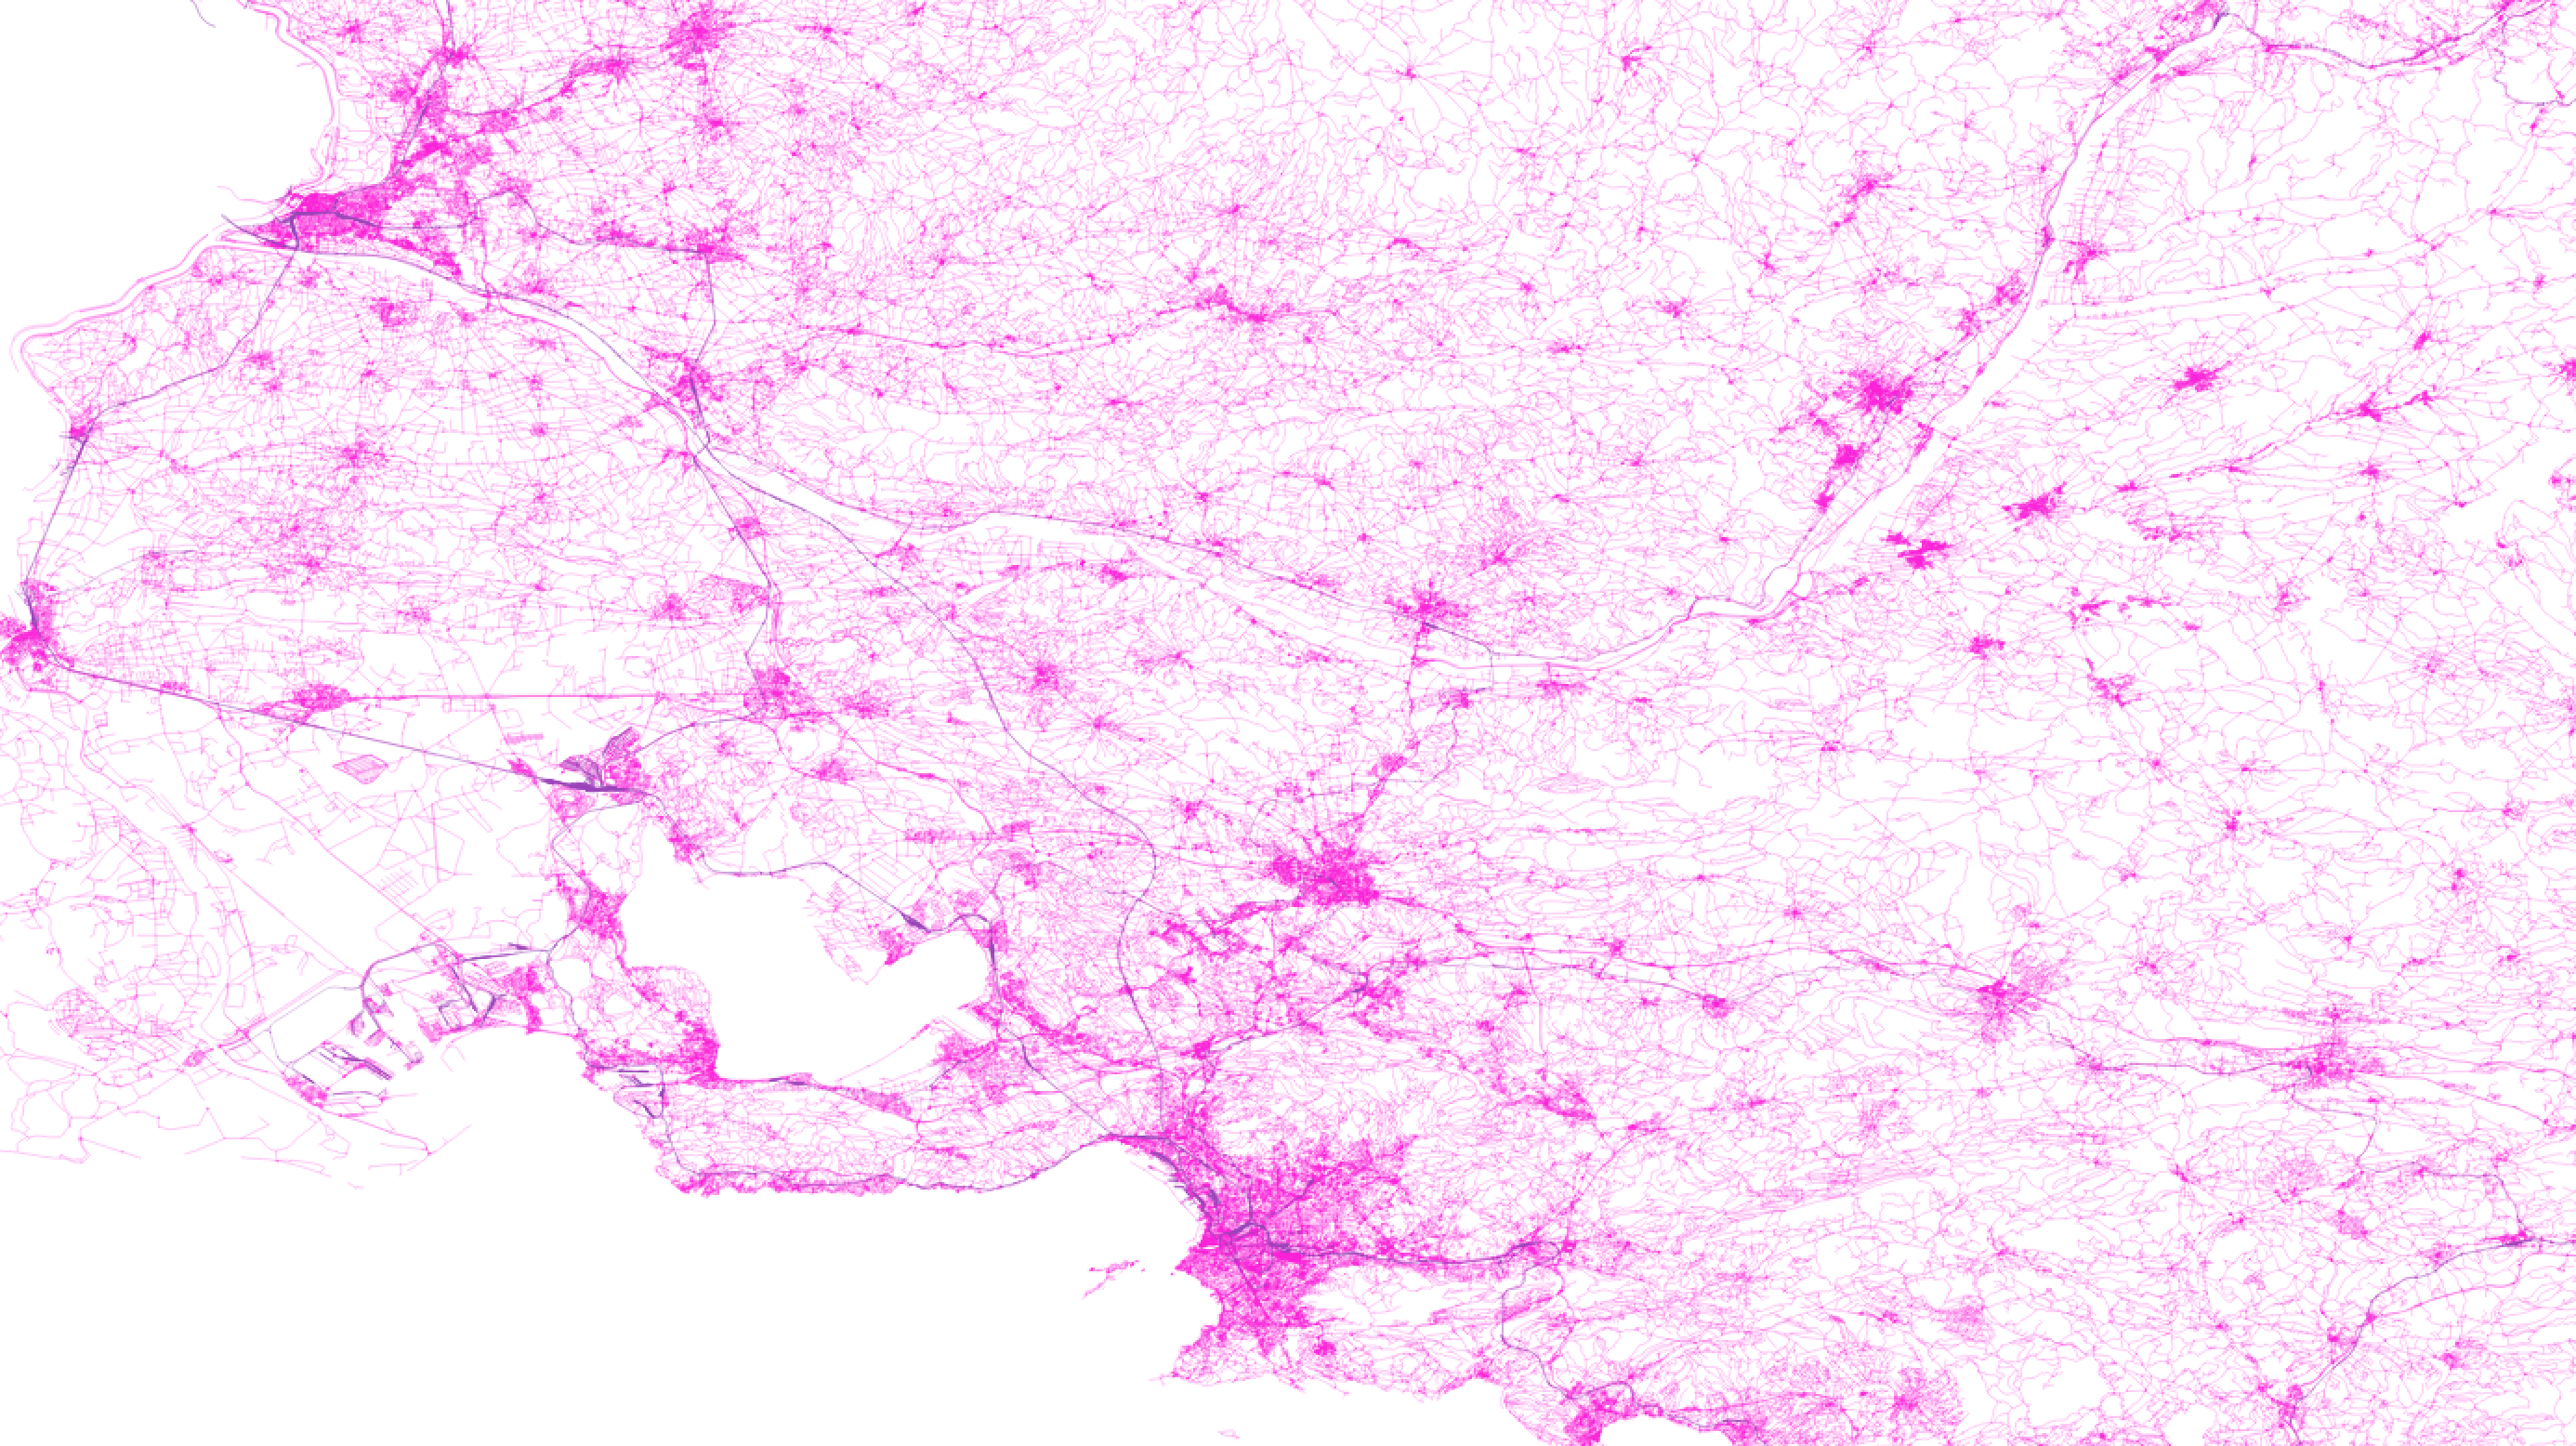
\includegraphics[width=1.2\textwidth]{figures/roadssouth.png}
	
	\footnotesize
\textit{Source: OpenStreetMap}


}


\sframe{Characterizing Road networks}{

%The structure of road networks both translates its past growth dynamics and has a significant impact on the sustainability of territories it irrigates.

% here extracts from Claire's work
% Lagesse, C., Bordin, P., & Douady, S. (2015). A spatial multi-scale object to analyze road networks. Network Science, 3(1), 156-181. -> nice picture Avignon

% La caracterisation des reseaux routiers, par exemples en termes de classification et dindicateurs topoliques, est liee a differents enjeux qui incluent la comprehnsion des dynamiques ppasses par la contingence de ces artefacts, amis qussi des questions futues liees a la soutenabilité des territoires qui'ils irriguent.
% les developpements recents, issus d'efforts interdispclinaires, incluent par exmeple ce travail de Claire Lagesse applique a la ville que v ous reconnaissaez bien, pour la definition de nouveau object a la pertineence thematique plus grande que les seuls entites des bases de donnes sans ontologie propre. (ex perso ballade avignon hier : vraie coherence thematique de l'objet "Way")

\textit{Multiple dimensions to characterize road networks}

\medskip

{
\centering
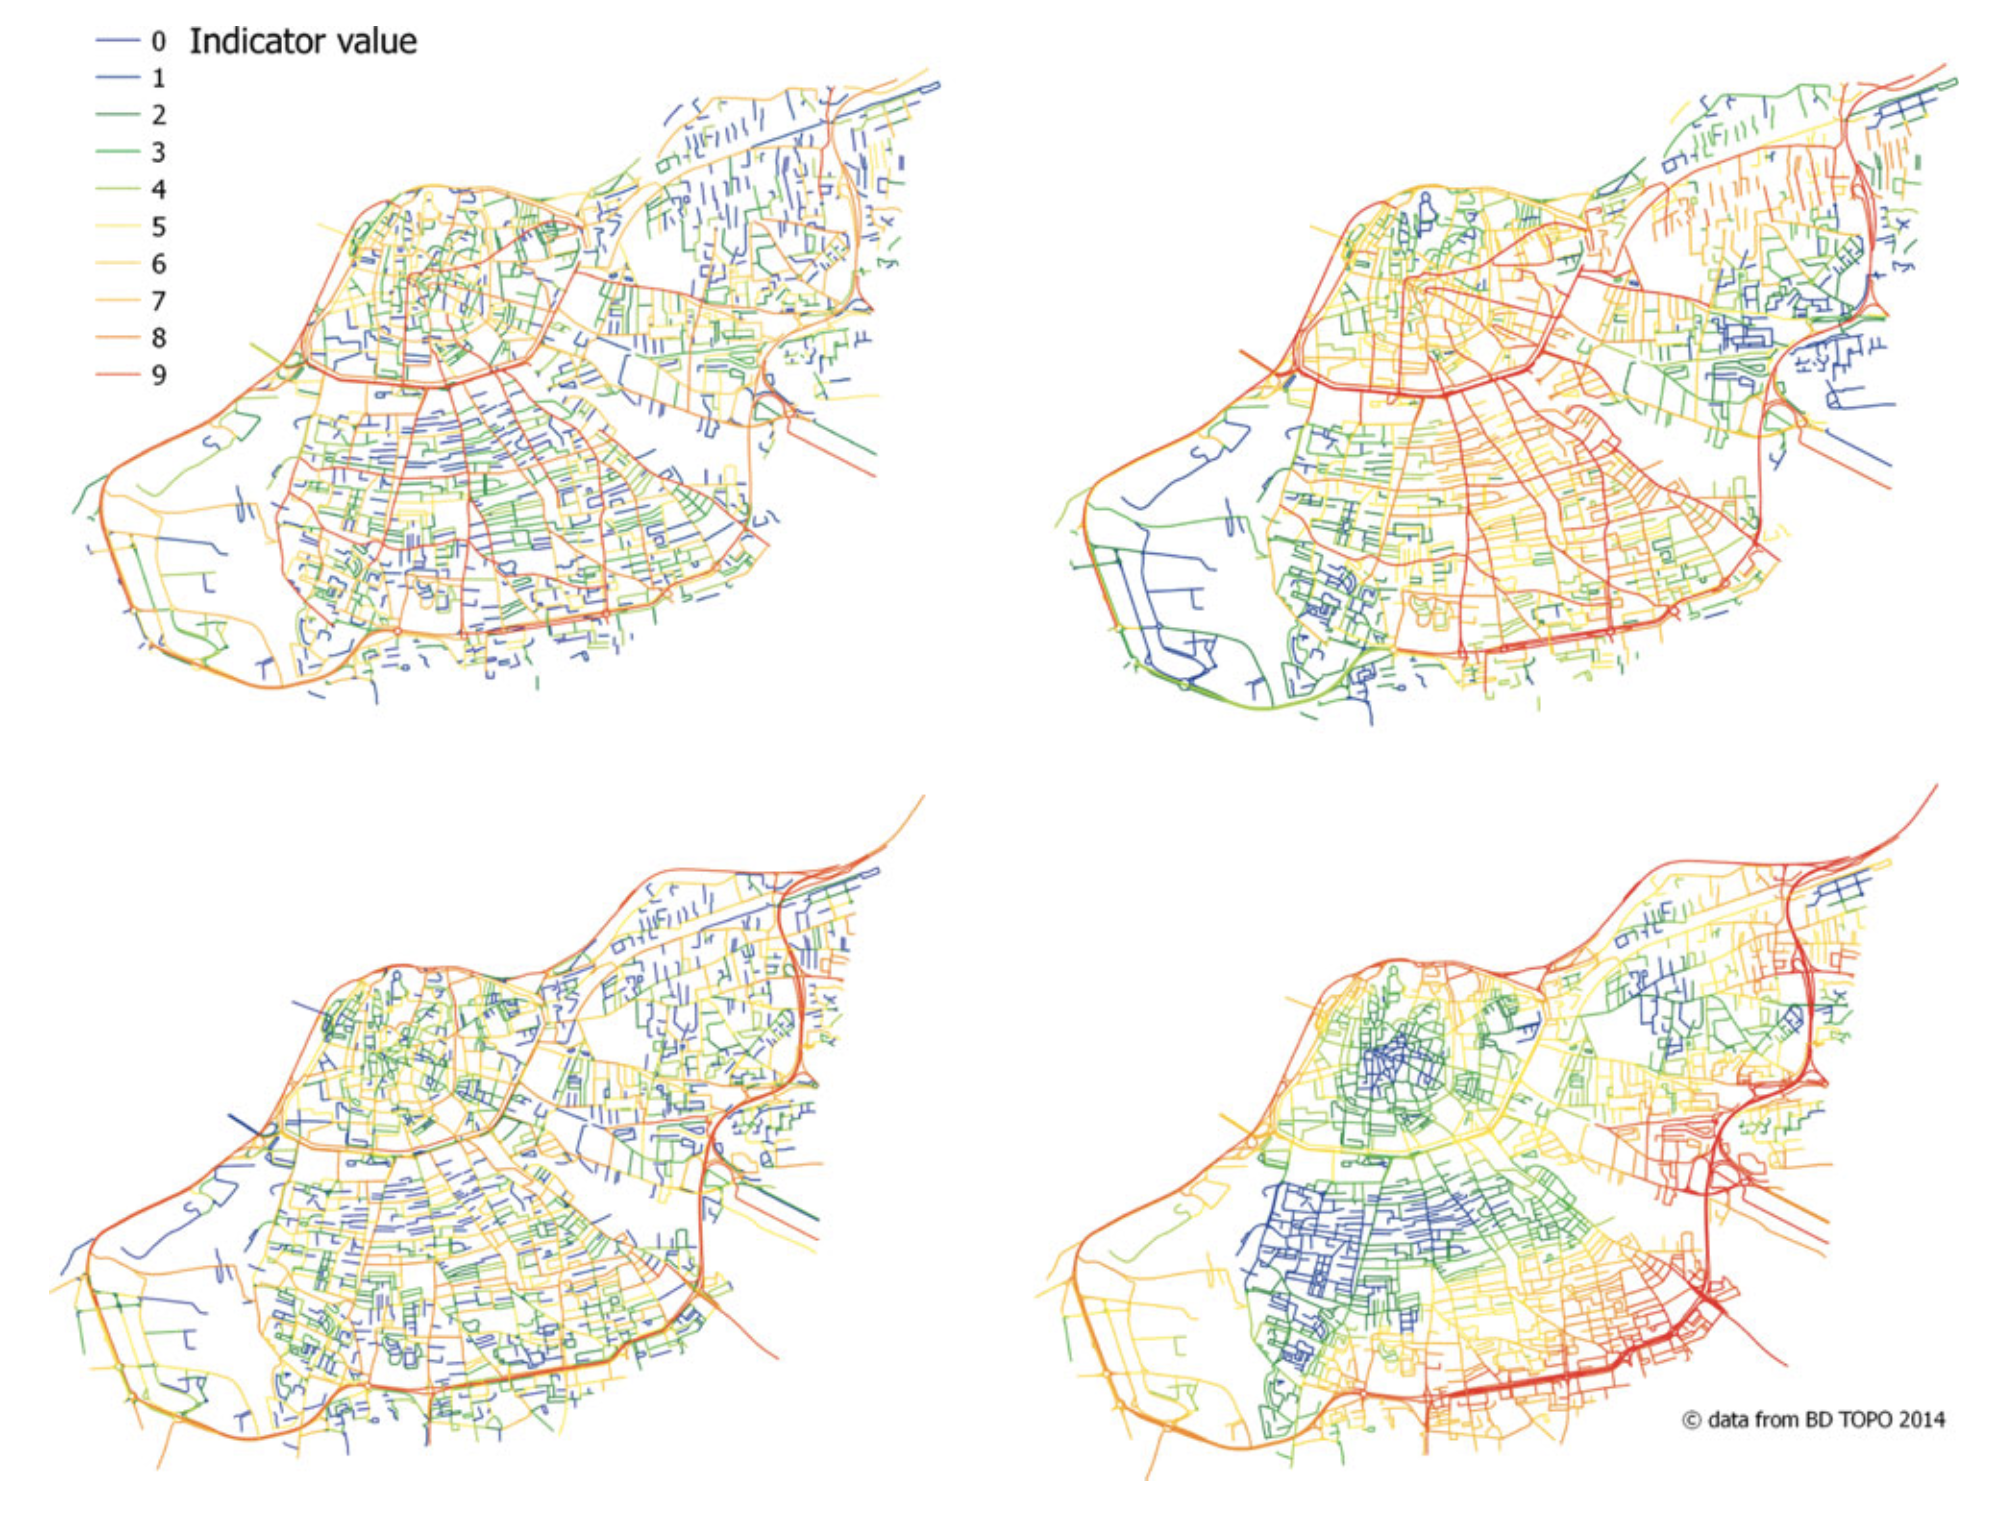
\includegraphics[width=\textwidth,height=0.7\textheight]{figures/avignon_claire.png}
}

\footnotesize

Lagesse, C., Bordin, P., \& Douady, S. (2015). A spatial multi-scale object to analyze road networks. Network Science, 3(1), 156-181. \cite{lagesse2015spatial}


}


\sframe{Network percolation}{

% A method to characterize topologies of these spatial networks is network percolation. Such approaches have been applied to the modeling of urban growth \citep{makse1998modeling} and to the analysis of street networks for example to extract endogenous urban regions \citep{arcaute2016cities} or to characterize the spatial morphology of point patterns \cite{huynh2018characterisation}.

% from monodimensional to multidimensional

% similar to 
%Cottineau, C., Finance, O., Hatna, E., Arcaute, E., & Batty, M. (2018). Defining urban clusters to detect agglomeration economies. Environment and Planning B: Urban Analytics and City Science, 2399808318755146.

% 

% parmi ces outils, la percolation a ete applique recemment aux reseaux routiers.
% en phyique, ce phenomene designe la traversee d'un milieu plus ou omins poreux par un fluide, et par exetnsion les processus pour l'attendre. En pariculier, nous l'entendrons au sens d'une occupation progressice des sites / connections des noeus d'un reseau, jusqu'a un etat critique ou l'ensemble de ceux-ci sont connectés (percolation threshold). [probailite de perco p_c]
% en particulier ppour letude des viulles
% des travaux relaticement anciens ont propose un phenomene de percolation locale correlation pour modeliser l'etalement urbain.
% plus recemment, et plsu proches des travaux des physiciens, une determination endoganee des regions urbaines a etet proposee par l'equipe du acvs en appliquant une heuristqiue de percolation aux reseaux routiers.
% ces methodes peuvent egalement servier a effecteur des statistqieus spatiales.
% nous porposons ici d;'etendre ces methodes en prenant en compte differentes dimensions urbaines, de la meme maniere que cottineau et al combine densite de population et flux de commuting pour definir les regoins urbaines.

\justify

\textbf{Network percolation: } \textit{progressive occupation/connection of nodes of a network} \cite{callaway2000network}

\bigskip

Application to the study of cities:

\begin{itemize}
	\item modeling urban growth \cite{makse1998modeling}
	\item endeogenous determination of regions \cite{arcaute2016cities}
	\item characterization of spatial point patterns \cite{huynh2018characterisation}
\end{itemize}

\bigskip

\textit{Towards complementary dimensions to condition road network percolation}

$\rightarrow$ similar to \cite{cottineau2018defining} to define urban areas

}





\sframe{Multidimensional percolation}{

% Existing heuristics however generally focus on a single morphological dimension of networks, and leave out the functional properties of urban systems \citep{burger2012form}.

% - why the relation between form and function, aka pop and network in our view is crucial
% - take into account in percolation
% - potential application : endogenous sustainable urban entities

% notre approceh reponde a la question ouverte du lien entre ofrme et fonction da`ns les systemes urbaine ;  et par ailleurs se base sur les interatcions entre reseaux te territoires poour fournire un proy de ce lien.
% nous propospns ainsi d'explorer une heuristique multi-dimensionnelle de la percolation qui prend en compte morplholohie urbaine et yopologie dy reseau routier ; nous l'appliquon pour caracterisere endogenement les regions urbaines.
% [rq : deux niveau de reseuax dans notree apporche : (mais en. fait comme souvent en geo ; ) le physique, et le abstraot que l'on construite a partir d'entites spatiales.


\justify

$\rightarrow$ Need to combine morphological and functional dimensions of cities \cite{burger2012form}

\medskip

$\rightarrow$ Interactions between networks and territories to capture the link between form and function \cite{raimbault2018caracterisation}; potential application to sustainability of urban systems

% research question


\bigskip
\bigskip

\textbf{Research objective : } \textit{Investigate a multi-dimensional percolation of territorial networks taking into account urban morphology and road network topology; endogenous characterization of urban regions.}

}



% \section{Method}

\sframe{Multilayer percolation}{

%This communication addresses such a gap by introducing a multi-dimensional percolation heuristic, which is analog to multilayer network percolation \citep{boccaletti2014structure}. Given discrete spatial fields, site percolation is operated between two cells given a threshold parameter for each dimension and a distance threshold.

% decrivons a presons de neniere stylisee l'algorithme utilise.
% le processus de peroclation initrial est deterministe, base sur la distance, met est prochess des random eulidian networks evoque hier par Alain Franc : si deux neouds sont a une distance d'un rayon critique r_0, ceux ci sont connectes par un lien.
% nous ajoutons alors sur chaque couche du reaseu un seul de peroclation qui determine si le neod peut etre prus en compte dqns le reseau de la couhce.
% par conjonction des contraintes, nous obtenus un reseau a unique couche dans laquelle simplement els composantes connexes donnent les clusters perfcolés.

\textit{Multi-dimensional network percolation heuristic, similar to multilayer percolation} \cite{boccaletti2014structure}

\bigskip


\centering
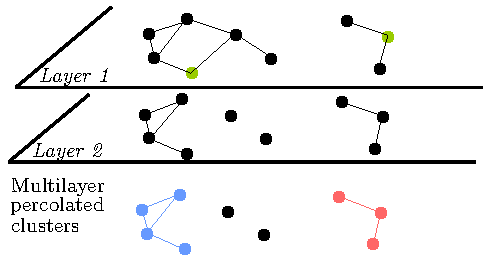
\includegraphics[width=0.8\textwidth]{figures/principle.pdf}


\bigskip

\raggedright

\textbf{Parameters: } percolation radius $r_0$, percolation thresholds $\theta_i$ for each layer


}




\sframe{Empirical data and variables}{

%We apply the heuristic to urban morphology and road network topology measures in Europe. More precisely, a grid with resolution 50km of population density morphology indicators and road network topology indicators, has been computed on spatial moving windows for all European Union by \cite{raimbault2018urban}. 

% Precisons a ppresent les objets geographiques a partir  desqueles nous allons construire le reseau.
% nous rappelns que nous cherchons a combiner prorpiete des territoires, que nous approximerons tres simplement par la districbution spatiale de la population, et propriete des reseaux routiers, que nous approximerons par des indicateirs topollogiques locaux.
% ces differentes caracteristqiues ont ete calucles, dans le cadre de ce travail de modelisation a l'echelle mesocscopique de la coevolution entre reseaux et cilles, sur les feentres glissantes de taille 50km poru l'ensemble de l'europe.
% nous en donnons ici l'illustration dans le cas de la France
% [several infos on different regimes etc]


\justify

\textit{Territorial indicators computed for Europe by \cite{raimbault2018urban}}

% here add maps to better visualize the spatial fields

\medskip

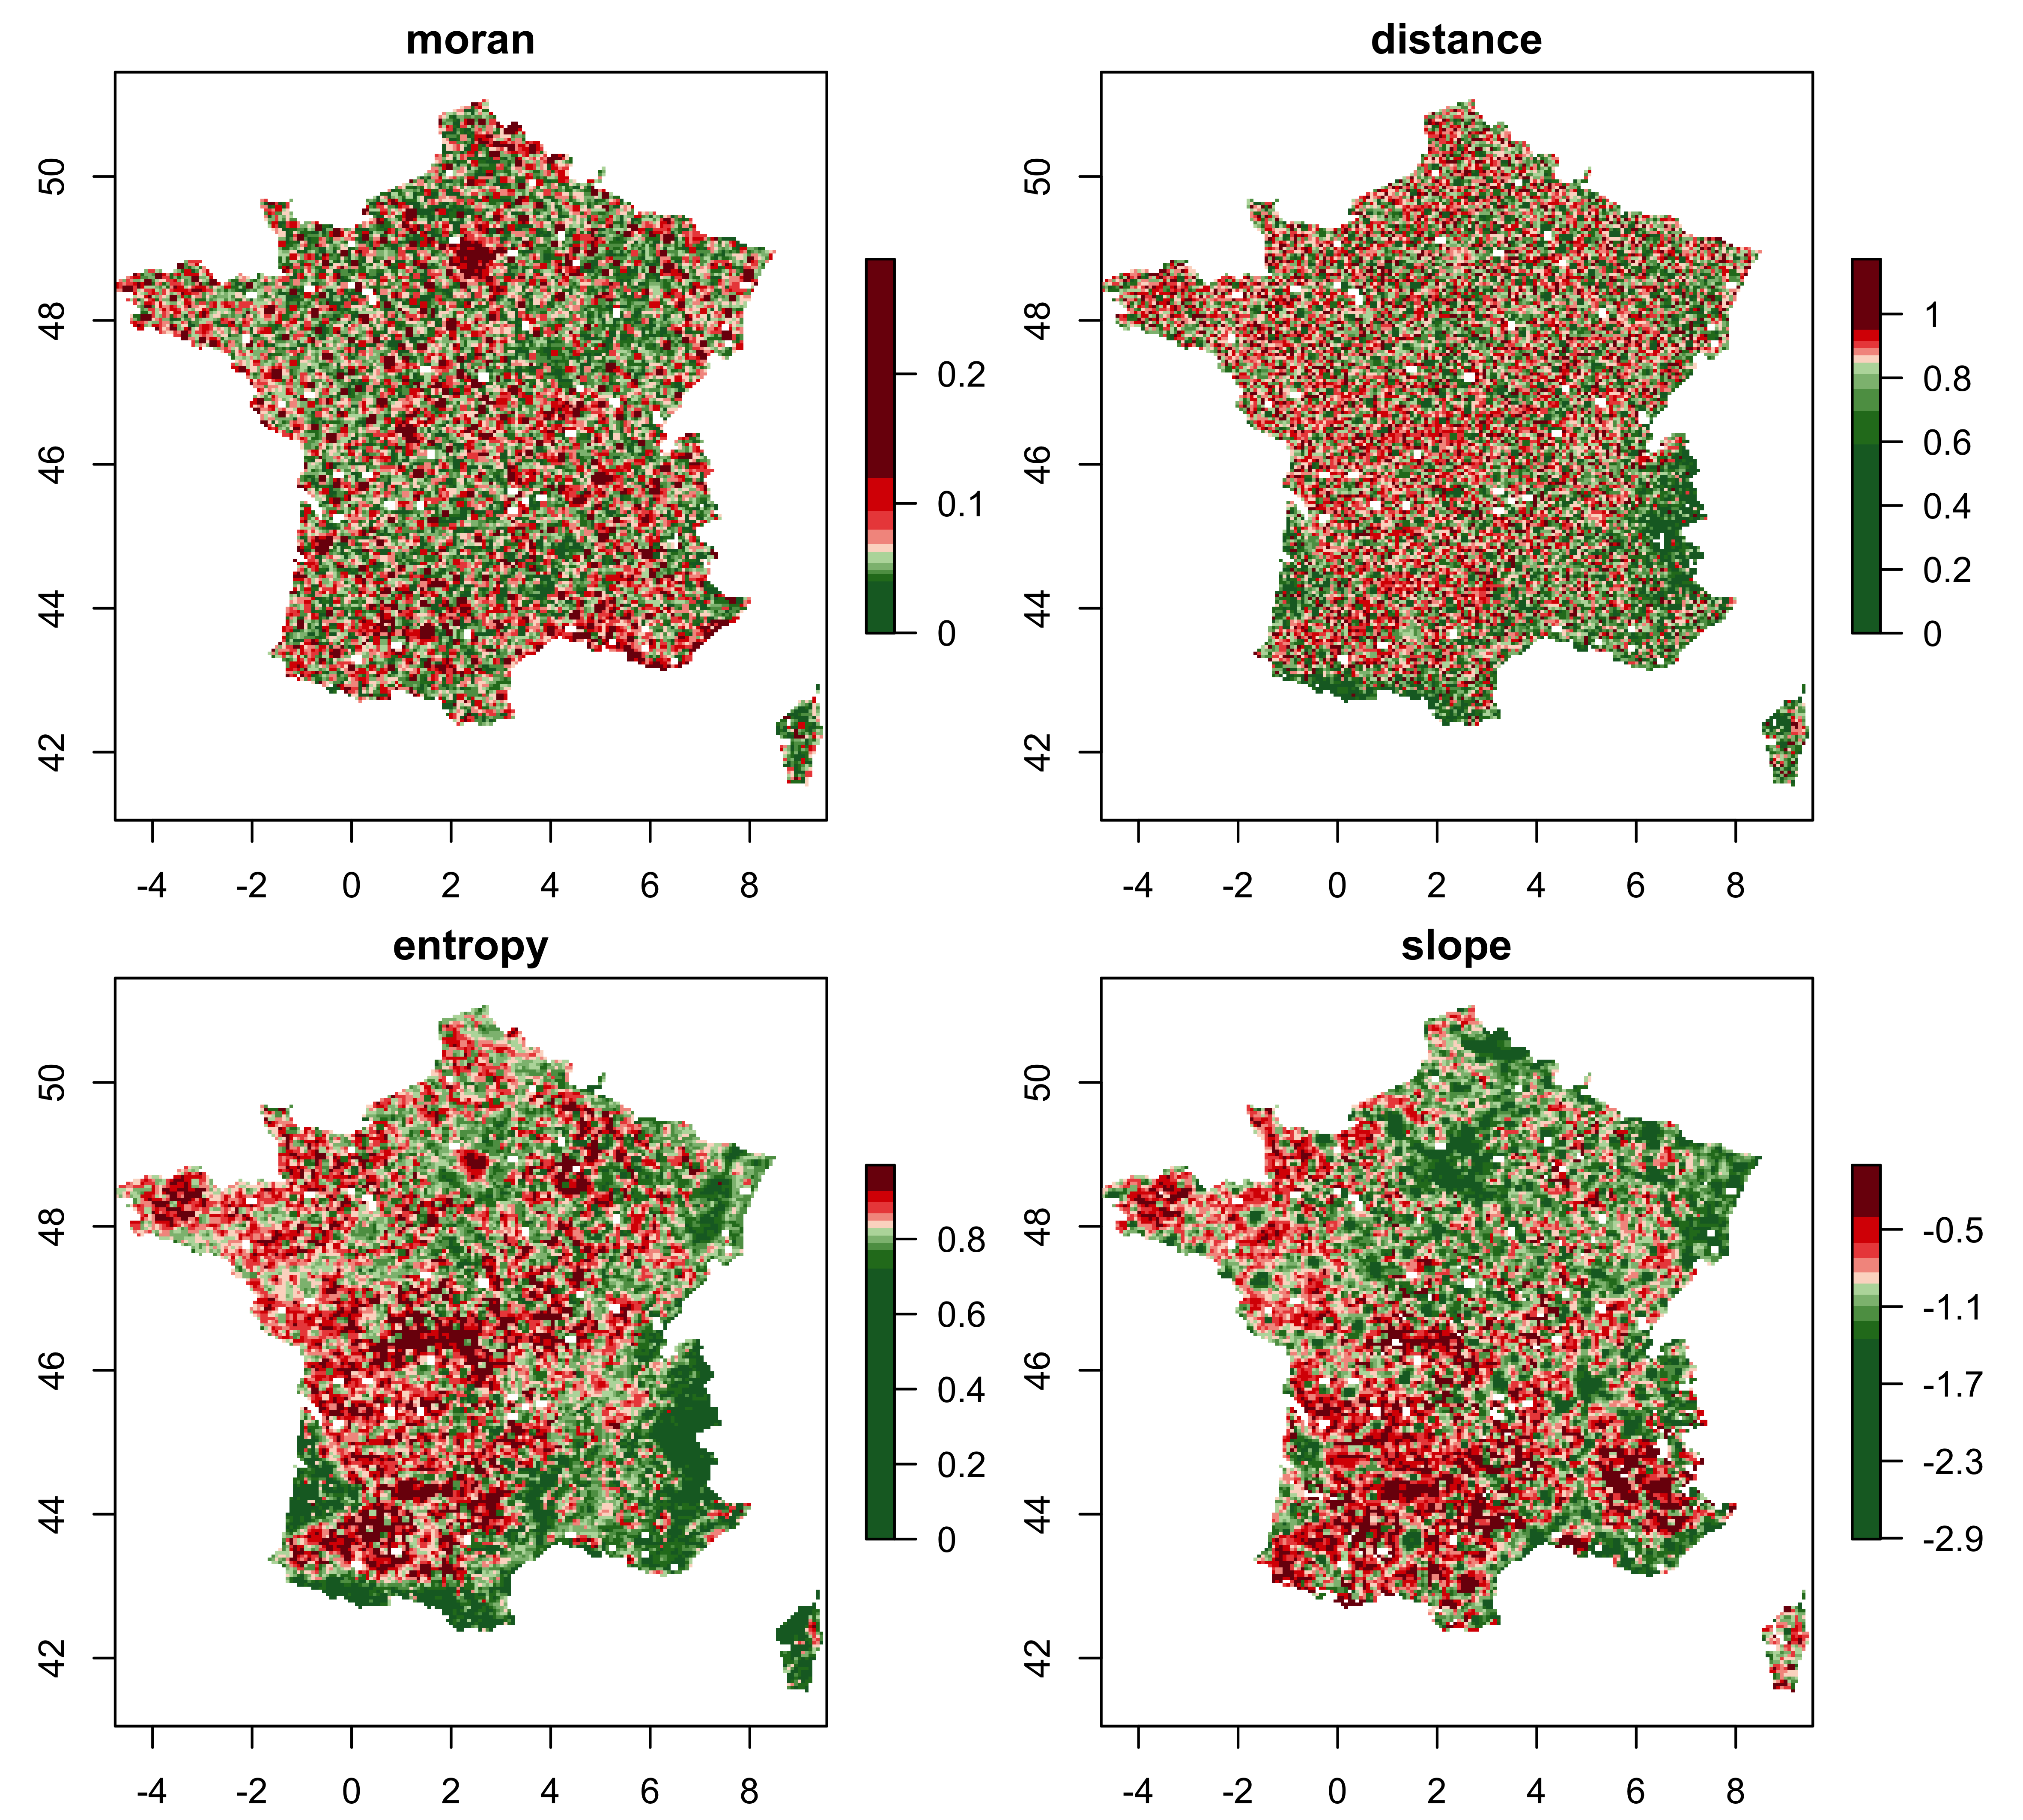
\includegraphics[width=0.49\textwidth]{figures/indics_morpho_discrquantiles.png}
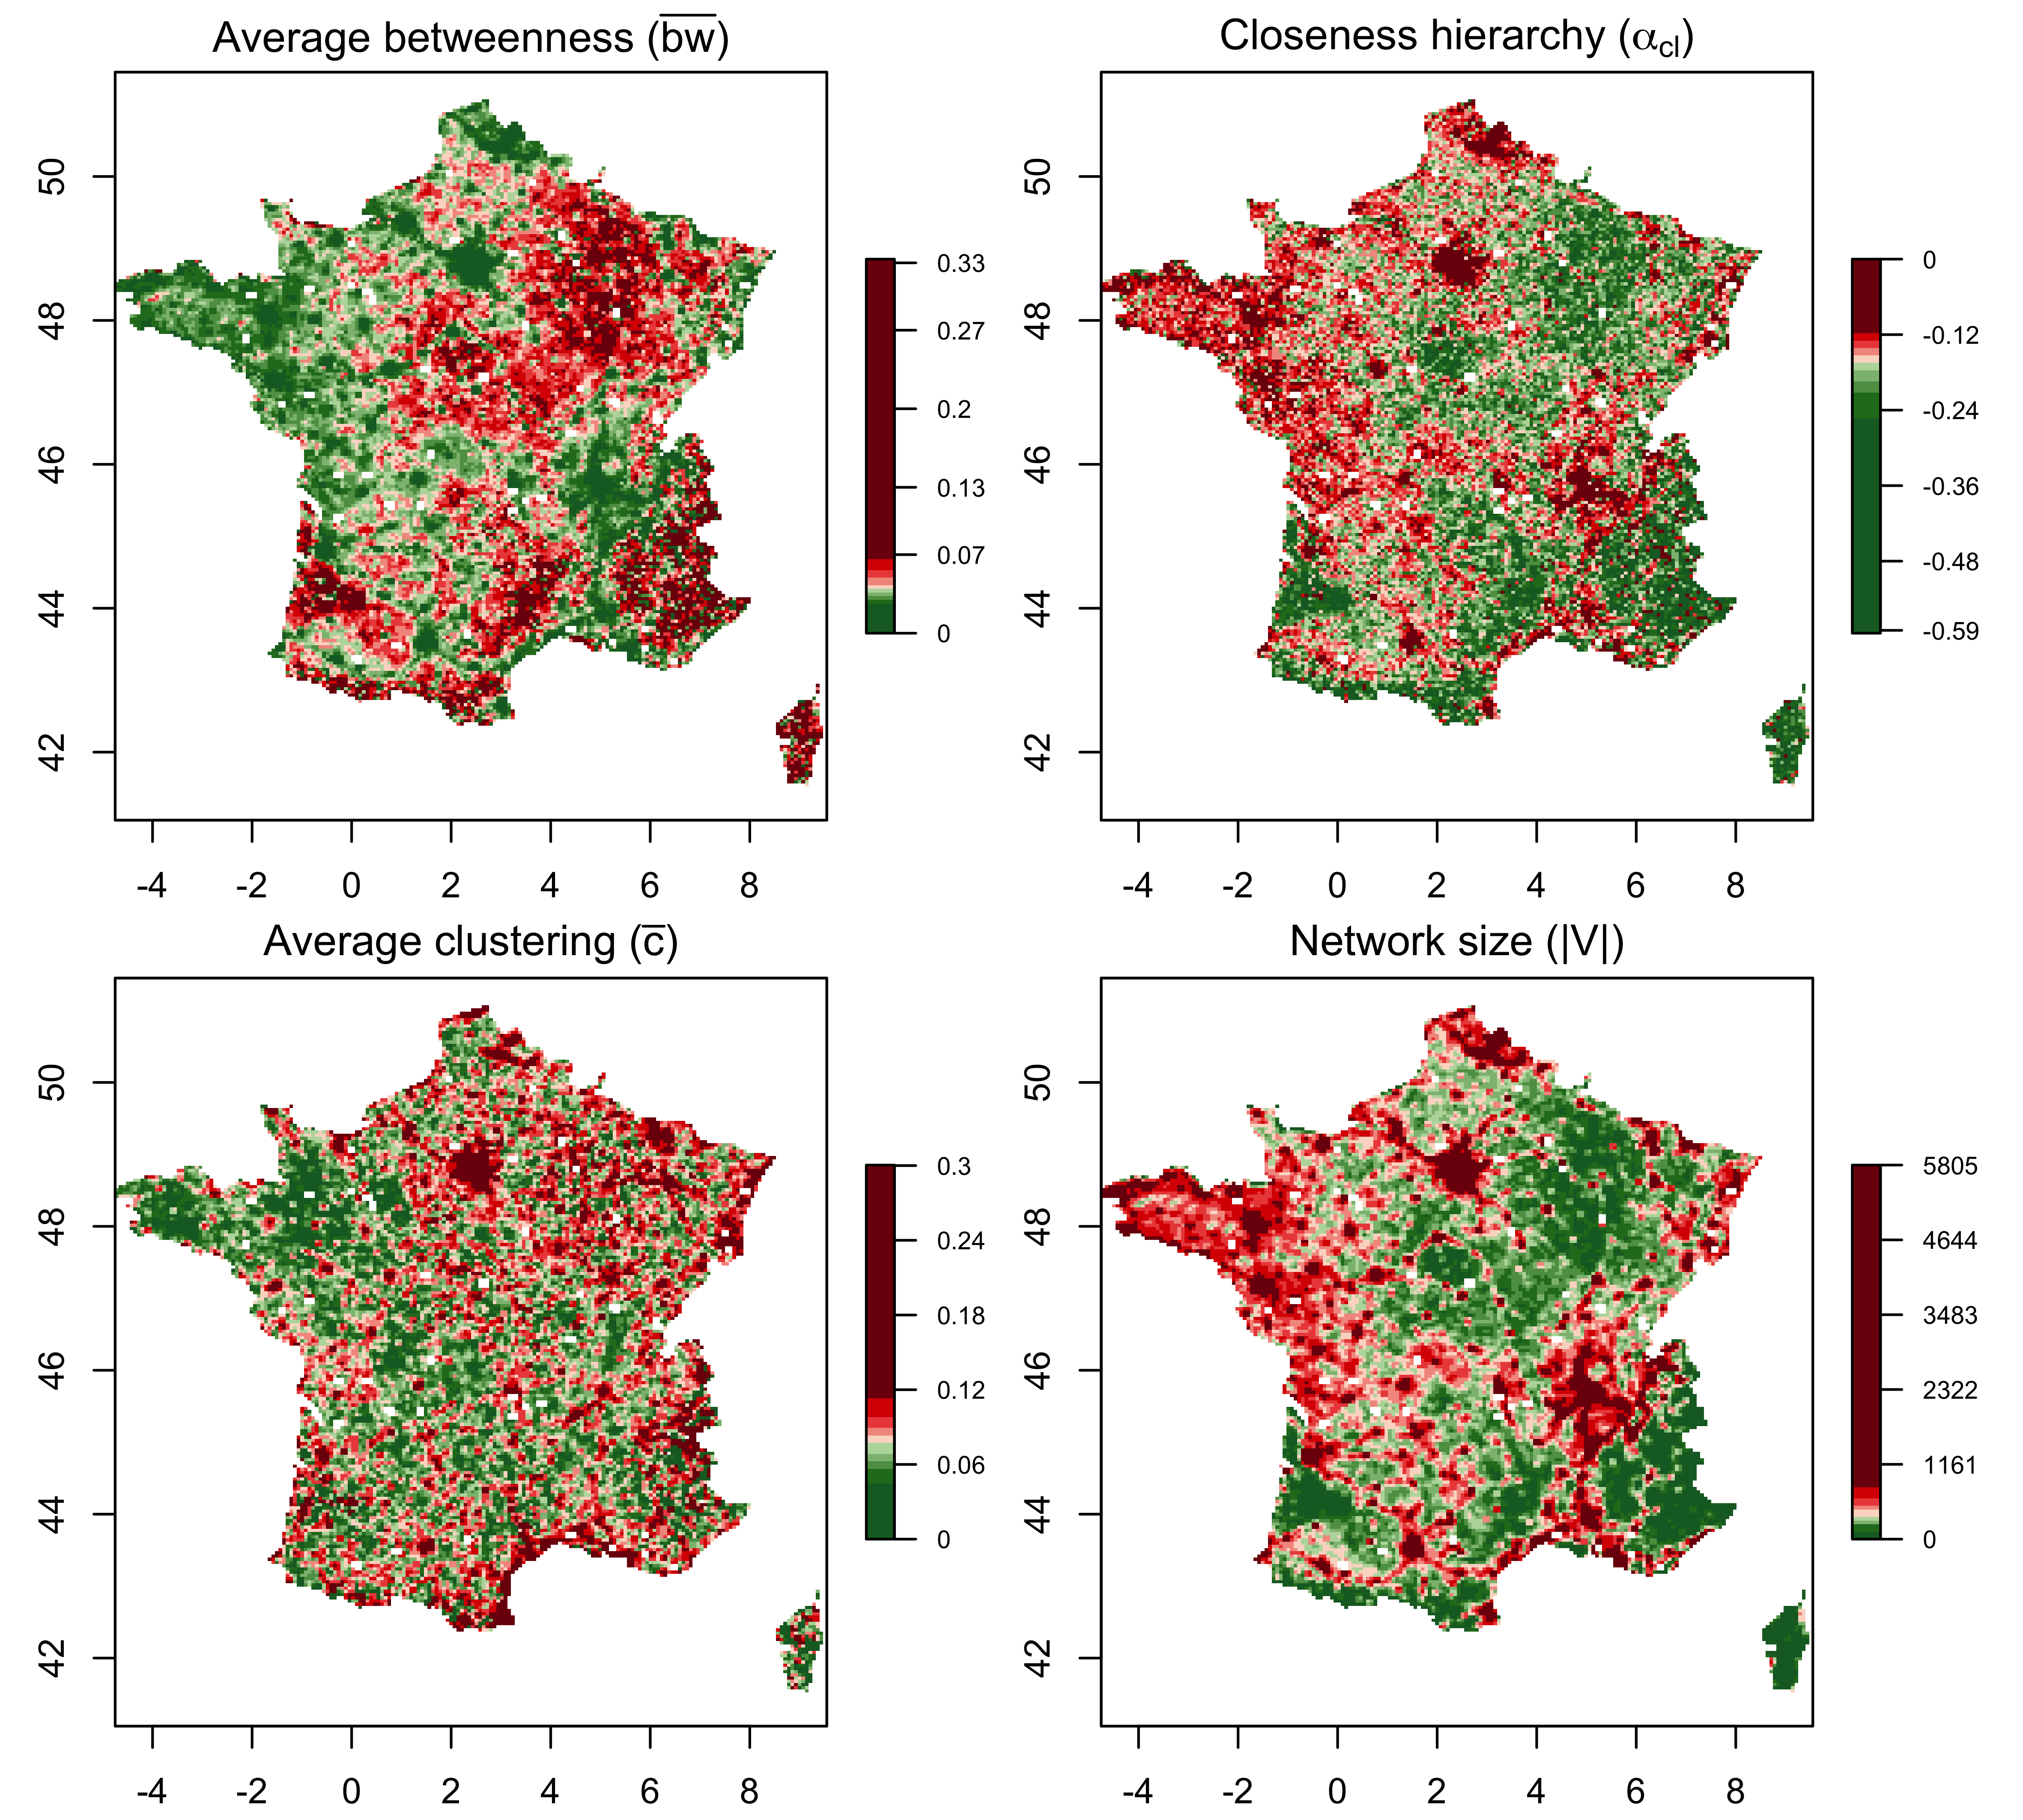
\includegraphics[width=0.49\textwidth]{figures/indics_network_en_areasize100_offset50_factor0_5.png}

\medskip

\textbf{Population distribution morphology} and \textbf{Network topology} (betweenness, closeness, clustering, efficiency, \ldots) computed on 50km spatial windows (Eurostat density grid and OpenStreetMap)

}

\sframe{Network construction}{

%We percolate the population density layer with a network characteristic layer, that we test among number of edges, number of vertices, cyclomatic number and euclidian efficiency, which capture functional properties especially for the two last.

% a partir de ces deux couches nous considerosn d'un [art la densite de population, d'autre part des proxus pour la densite ou perdormance du reseau ; avce les paramteres associes.
% la logique geographique derriere cela est liee a la premiere loi de Tobler : deux lieus proches etc  ; ajoute a la logique de la masse (loi de gravite), mais selon different aspects du reseau (car difficile de savoir quelle dimenion a priori jouera le role "equivalent" d'une densite de population : autant laisser libre et explorer plutot que de fixer arbitrairemenbt - maxime d'un computational scientist converti, bien sur.
% en pratqiuem nous contruison le reseau correspondant et isolns ses composantes connexes.
% descirption du plan d'explericence.


\justify

\textbf{Two layers: } population density (threshold $\theta_P$) and network characteristics (threshold $\theta_N$) taken among \{Number of edges, Number of vertices, Cyclomatic number $\mu$, Euclidian efficiency $v$ \}; percolated with a radius $r_0$

% banos2012towards

\bigskip

\textbf{Rationale: } \textit{two locations will be in relation if they are close, have a high population density and given network characteristics.}

% note : euclperf should be minimized whereas other maximized : issue ?

\bigskip


\textbf{Implementation: } construction of a single layer spatial network given the condition on the two layers and distances, from the 5km resolution indicators spatial field; extraction of connected components.


\bigskip

\textbf{Experience plan: } grid sampling for $r_0,\theta_P,\theta_N$ and network variables; additional gravity potential parameters $\gamma,d_0$ (detailed after)

$\rightarrow$ 4800 parameter points

%We systematically explore the clusters obtained for 840 parameter configurations. 

% + explain openmole -> later in potential developments

}





\sframe{Results: endogenous mega-regions}{

%Maps reveal that most configurations resemble the actual distribution of European mega-city regions, which are functionally integrated polycentric urban areas \citep{hall2006polycentric}. 

% les rsultats sont particulierement interessantm puiqaue ceratines valuers de apremtres menest a des configurations connues par lkes geographesm celles des mega-cities regions
% [rq : affirnation arbitraire iuci car pas evidence-based, il faudrait comp systematique etc , le probeleme vcest que meme pas de liste avec consensus sur l'obejct, comme soubent en geo>...]
% du coup "visuellemtn" randstad, rehinrhuhrm, rehinmainm London, Paris, Manchester Leeds,
%

\justify

\vspace{-0.4cm}
\textit{Extraction of endogenous polycentric mega-city regions \cite{hall2006polycentric}}

\medskip

\centering

% note : forgot r_0 in figs
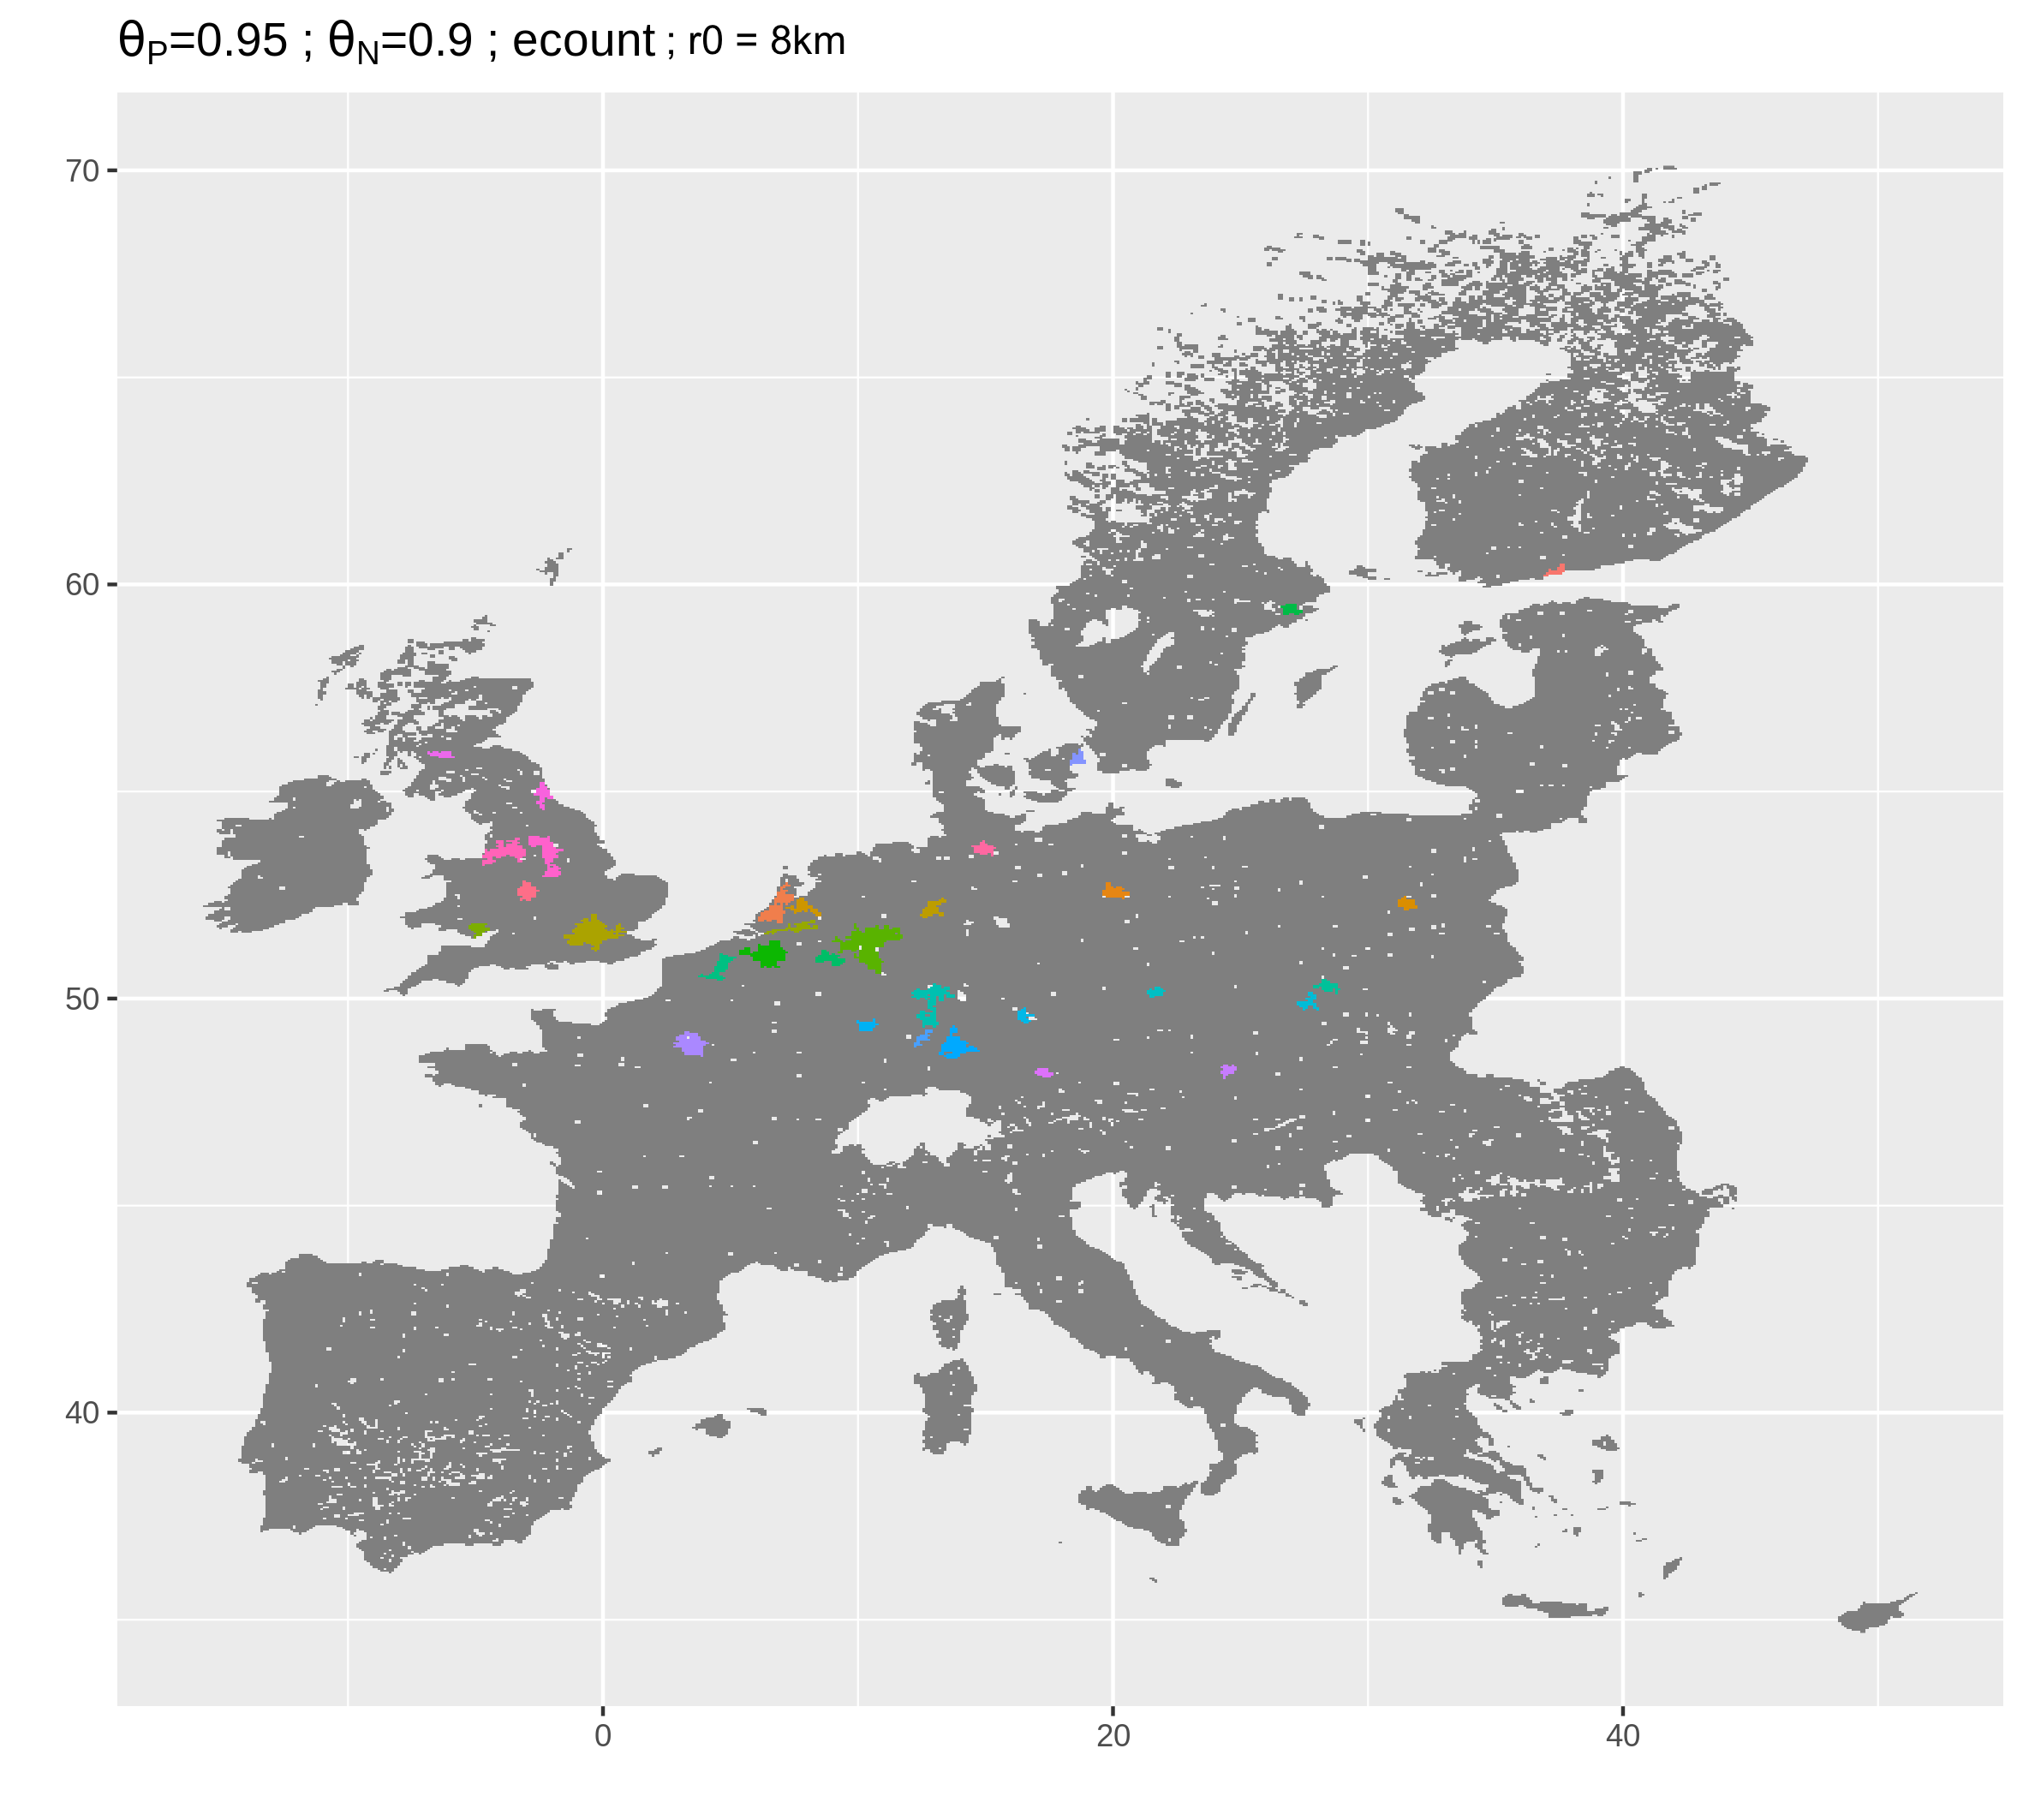
\includegraphics[width=\textwidth,height=0.9\textheight]{figures/totalPop4183694_00056402_ecount850_radius8000.png}


}

\sframe{Different endogenous morphologies}{

% TODO for the paper : check effect of adding network threshold : methodo info on multilayer percol in itself

\hspace{-0.5cm}
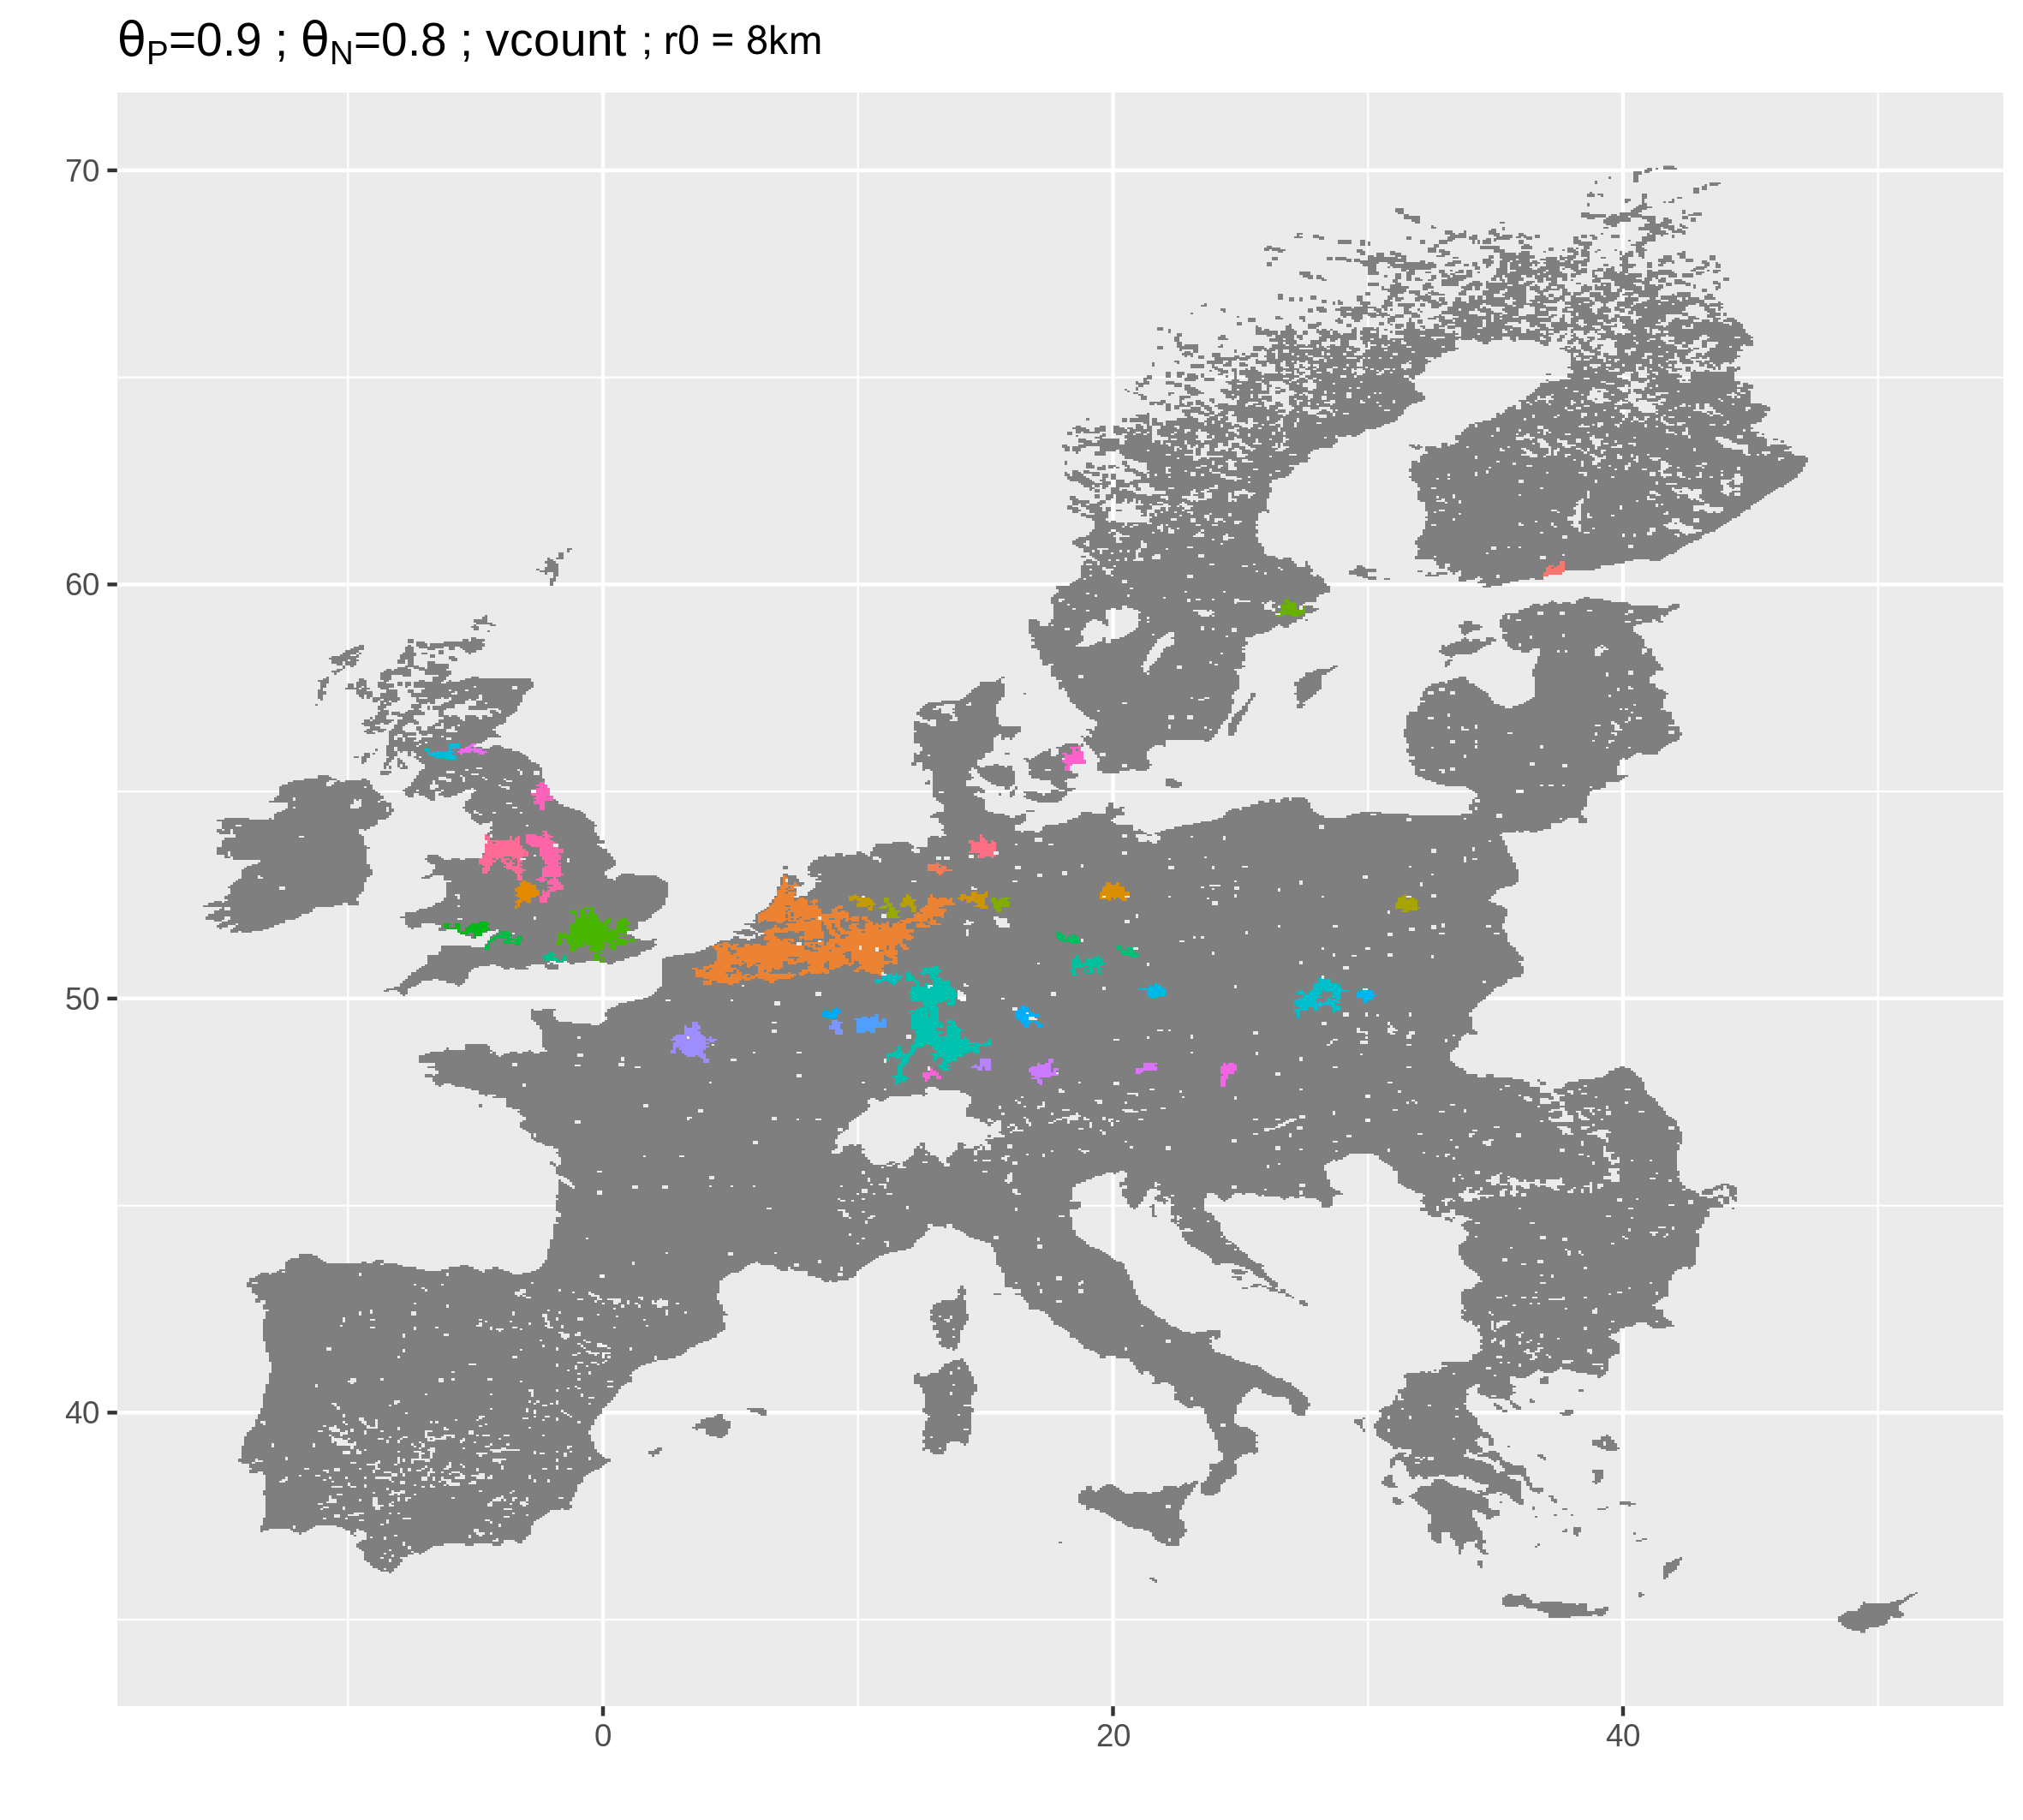
\includegraphics[width=0.52\textwidth]{figures/totalPop2219780_36719597_vcount378_radius8000.png}
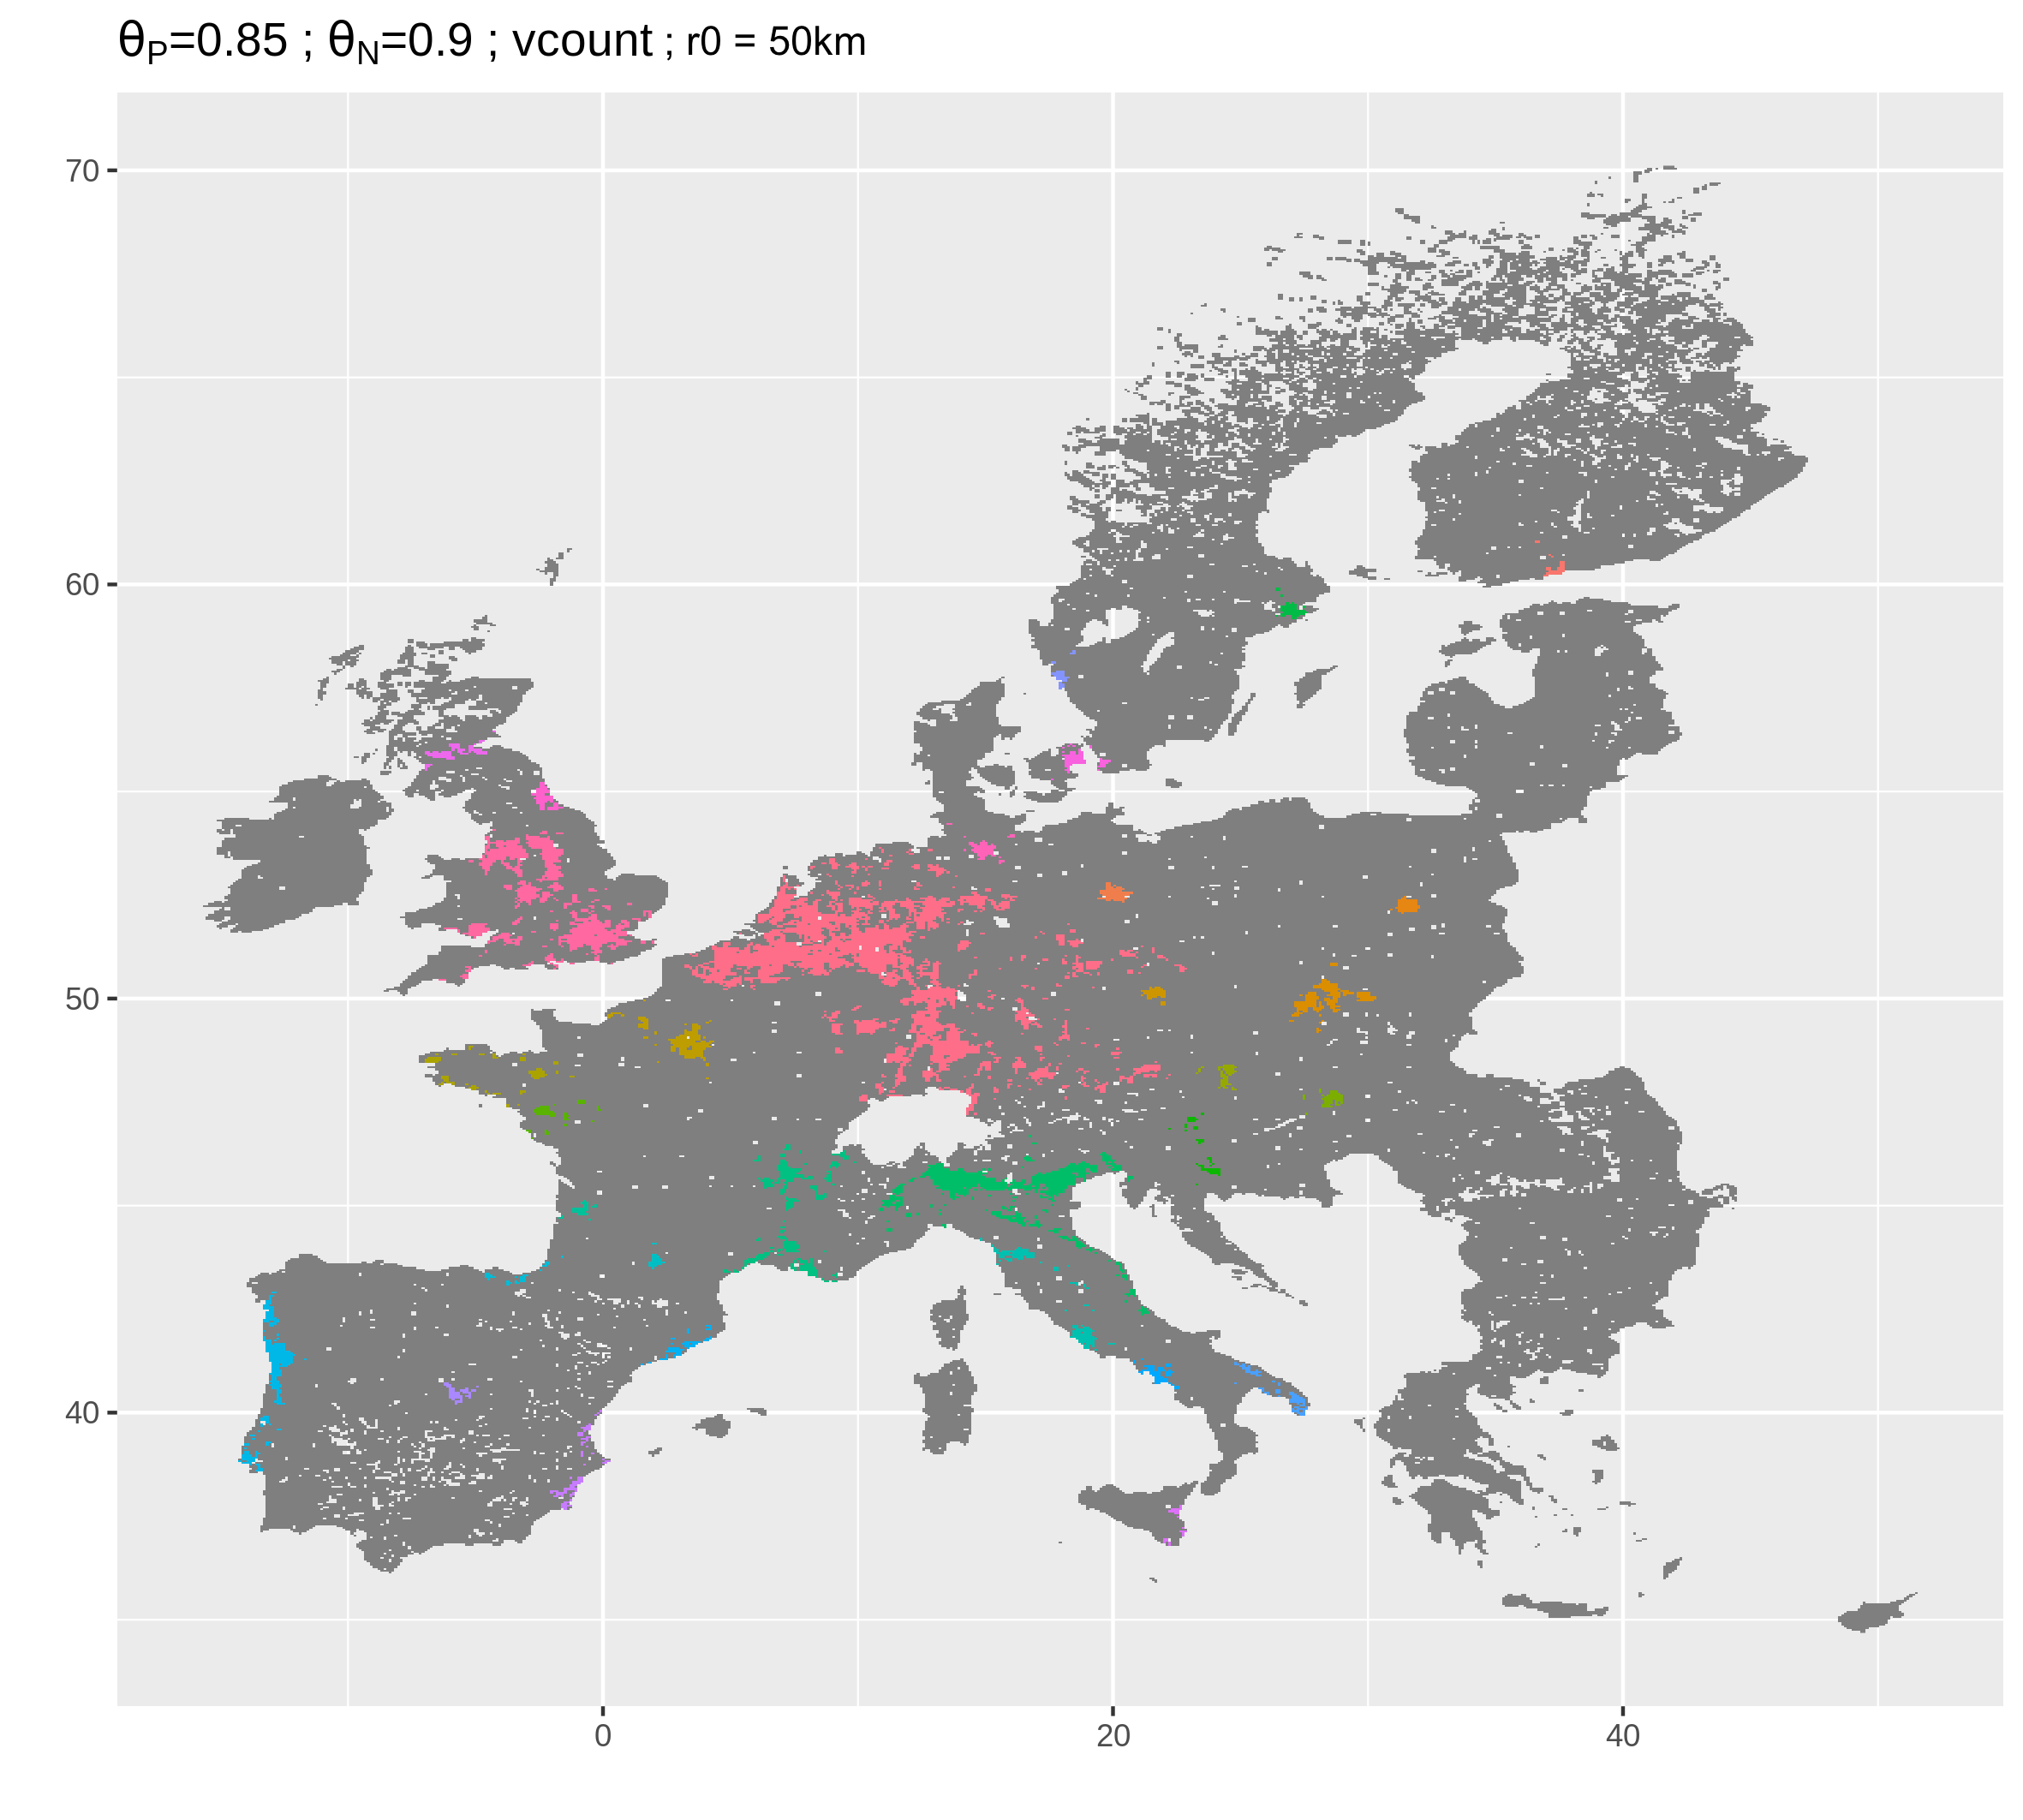
\includegraphics[width=0.52\textwidth]{figures/totalPop1474347_36891685_vcount595_radius50000.png}

}

\sframe{Characterizing sustainibility}{

% We use this endogenous definition of regional urban systems the percolation algorithm produced to evaluate their sustainability, in terms of conflicting objectives of economic integration and greenhouse gases emissions. Applying a gravity model to each region, we estimate transportation flows within each and extrapolate emissions by coupling with the Edgar emission database \citep{janssens2017edgar} and economic activities with a scaling law of population.

% explain indicators : convex hull.

\justify

\textbf{Application: } sustainability indicators for the endogenous urban regions; proxys for two conflicting dimensions: GHG emissions and economic integration \cite{viguie2012trade}.

\bigskip

\textbf{Data: } EDGAR database for GHG emissions (v4.3.2) 

\cite{janssens2017edgar}

\bigskip

\textbf{Estimation: } Abstract flows approximated with a gravity model

\[
\phi_{ij} = \left(\frac{v_i v_j}{(\sum_k v_k)^2}\right)^\gamma \cdot \exp\left(\frac{-d_{ij}}{d_0}\right)
\]

where $v_k$ are either effective local GHG emissions or population (economic activity scaling law of population \cite{bettencourt2007growth})

\medskip

$\rightarrow$ sum of flows within the geographical span of the cluster (convex hull) approximate potential emissions and economic activity


}

\sframe{Pareto fronts for sustainability}{

%  We show therein that different population, network and distance thresholds yield different performances in terms of sustainability, exhibiting a Pareto front. This suggests policies in terms of regional integration to increase the sustainability of mega-city regions.

\textit{Superposing Pareto front for observed population and emissions, on all clusters.}

\centering

\medskip

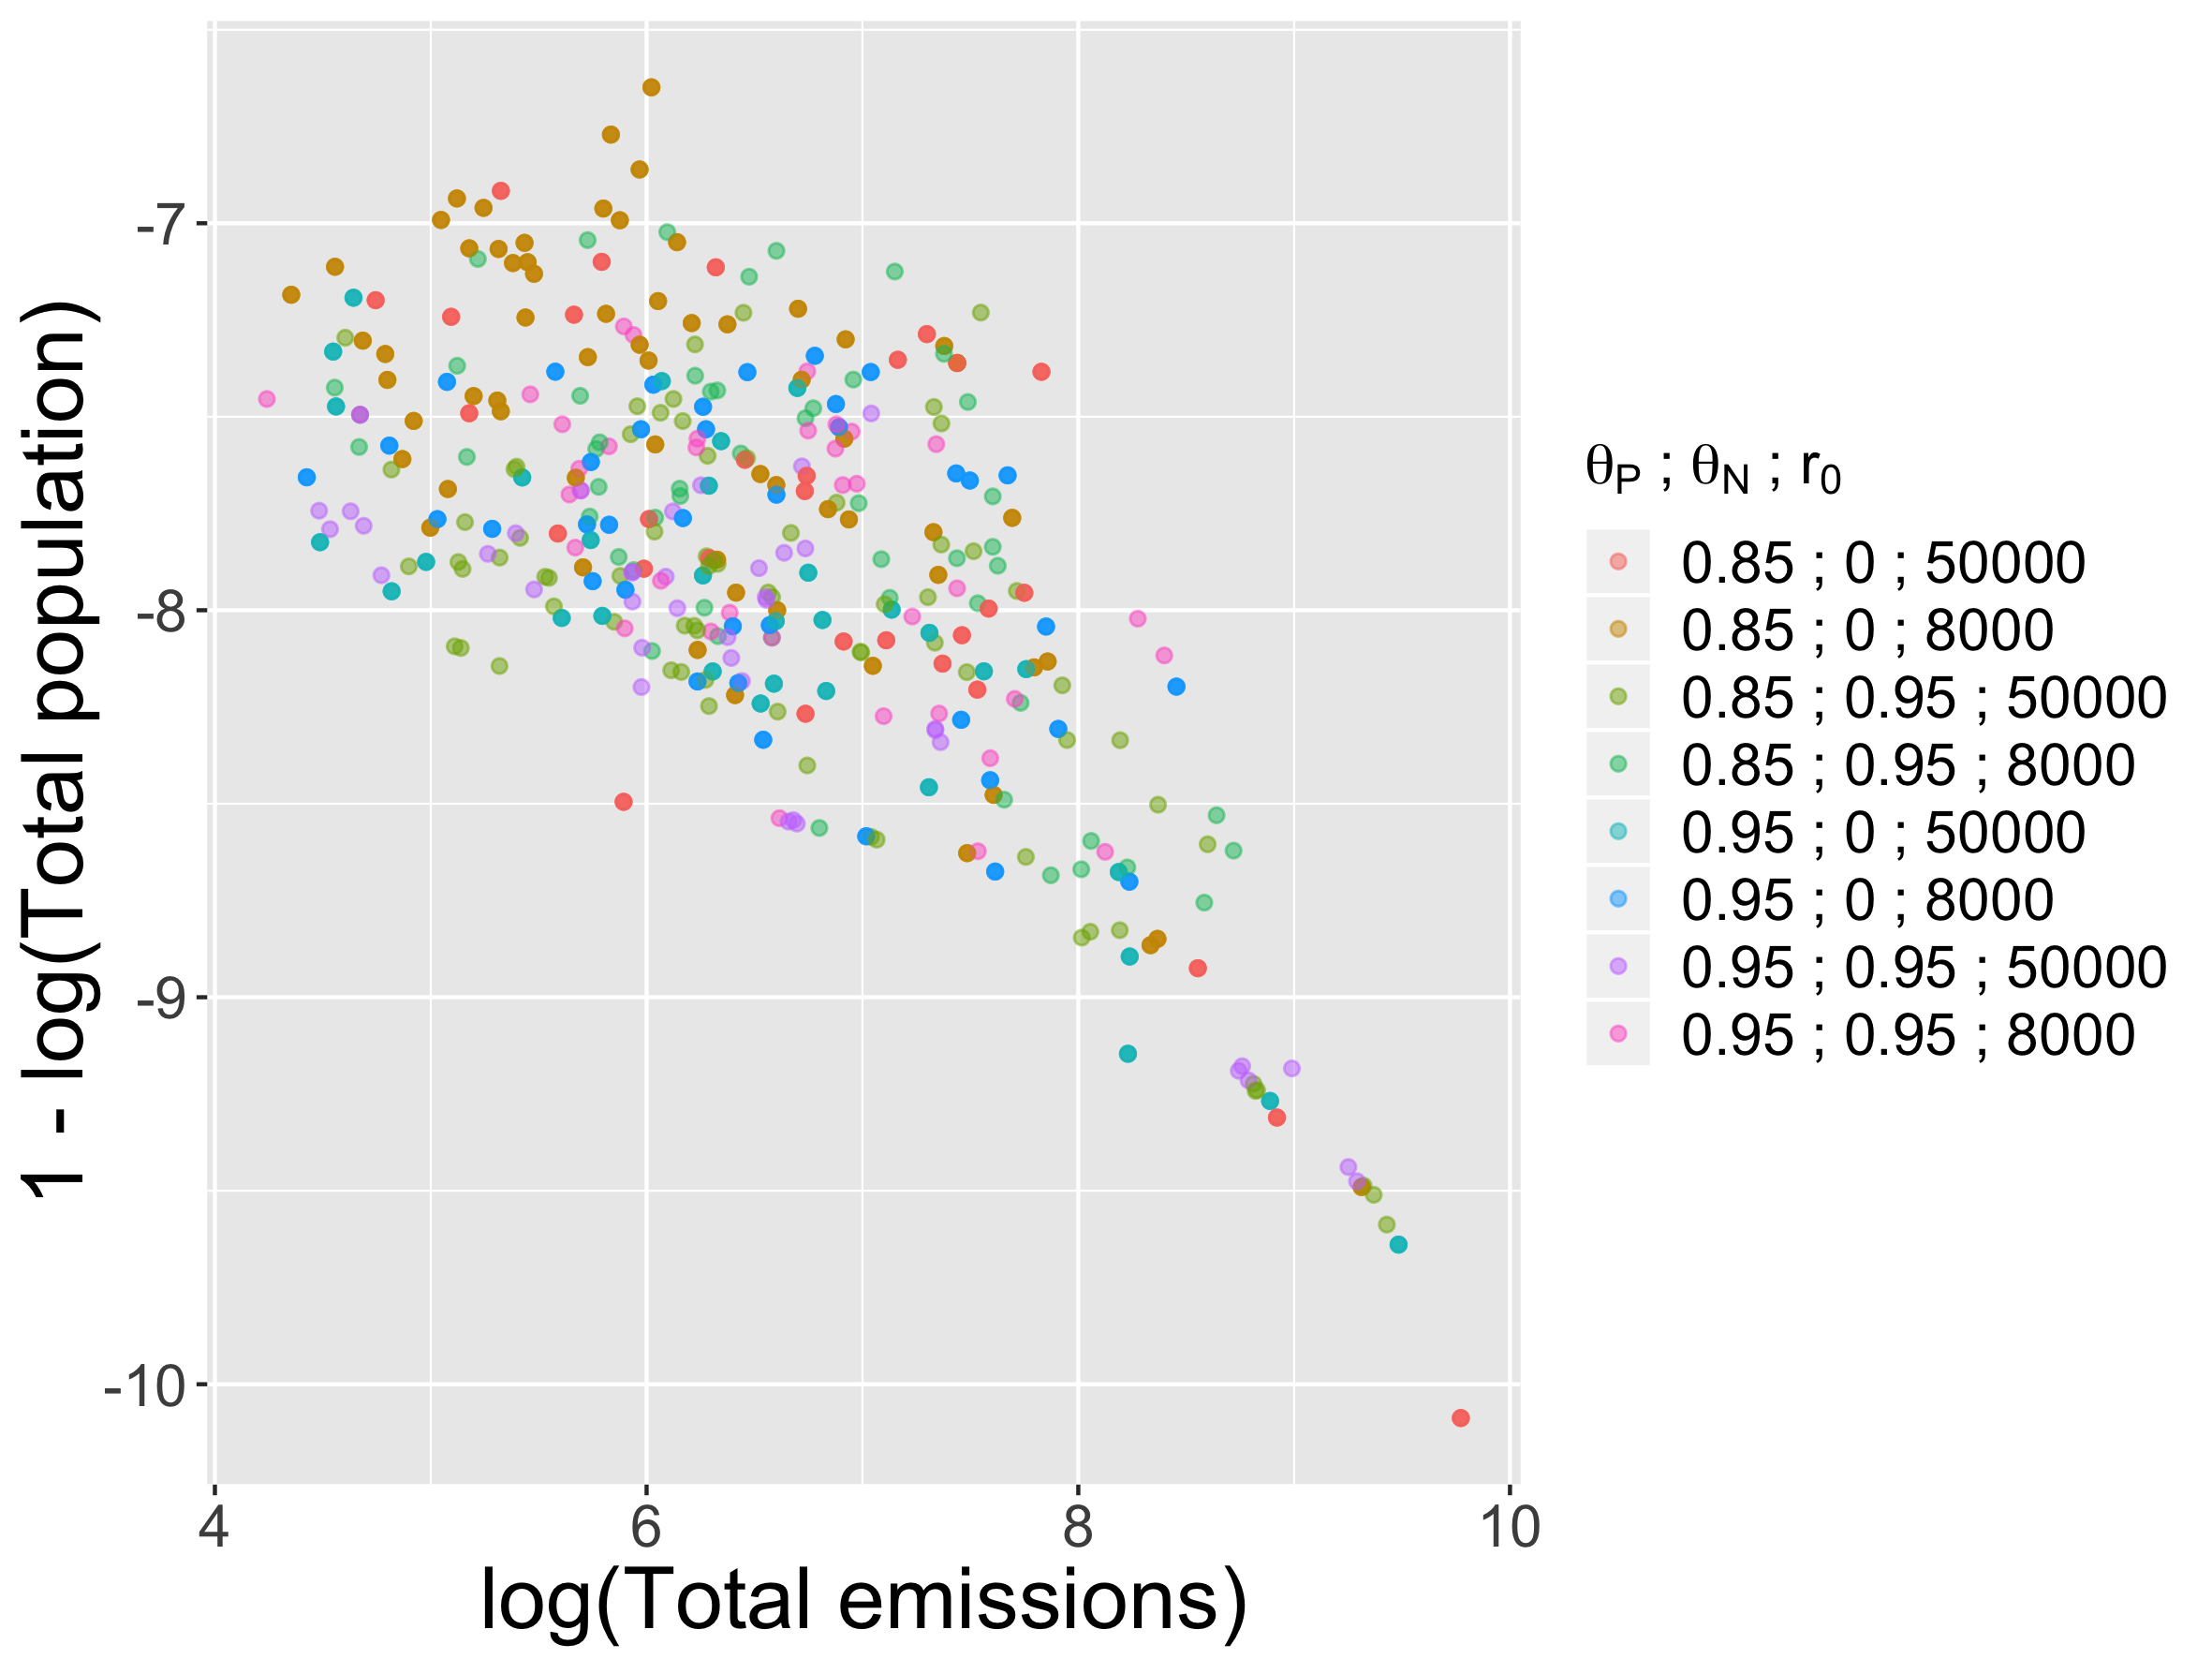
\includegraphics[height=0.8\textheight]{figures/full_effective_pareto.png}

% -> full fronts in reserve slide

}

\sframe{Pareto fronts for aggregated indicators}{

\textit{Aggregated sustainability indicators suggest some configurations are more Pareto efficient (high $\gamma$ regime, activities with high added value).}

\centering

\medskip

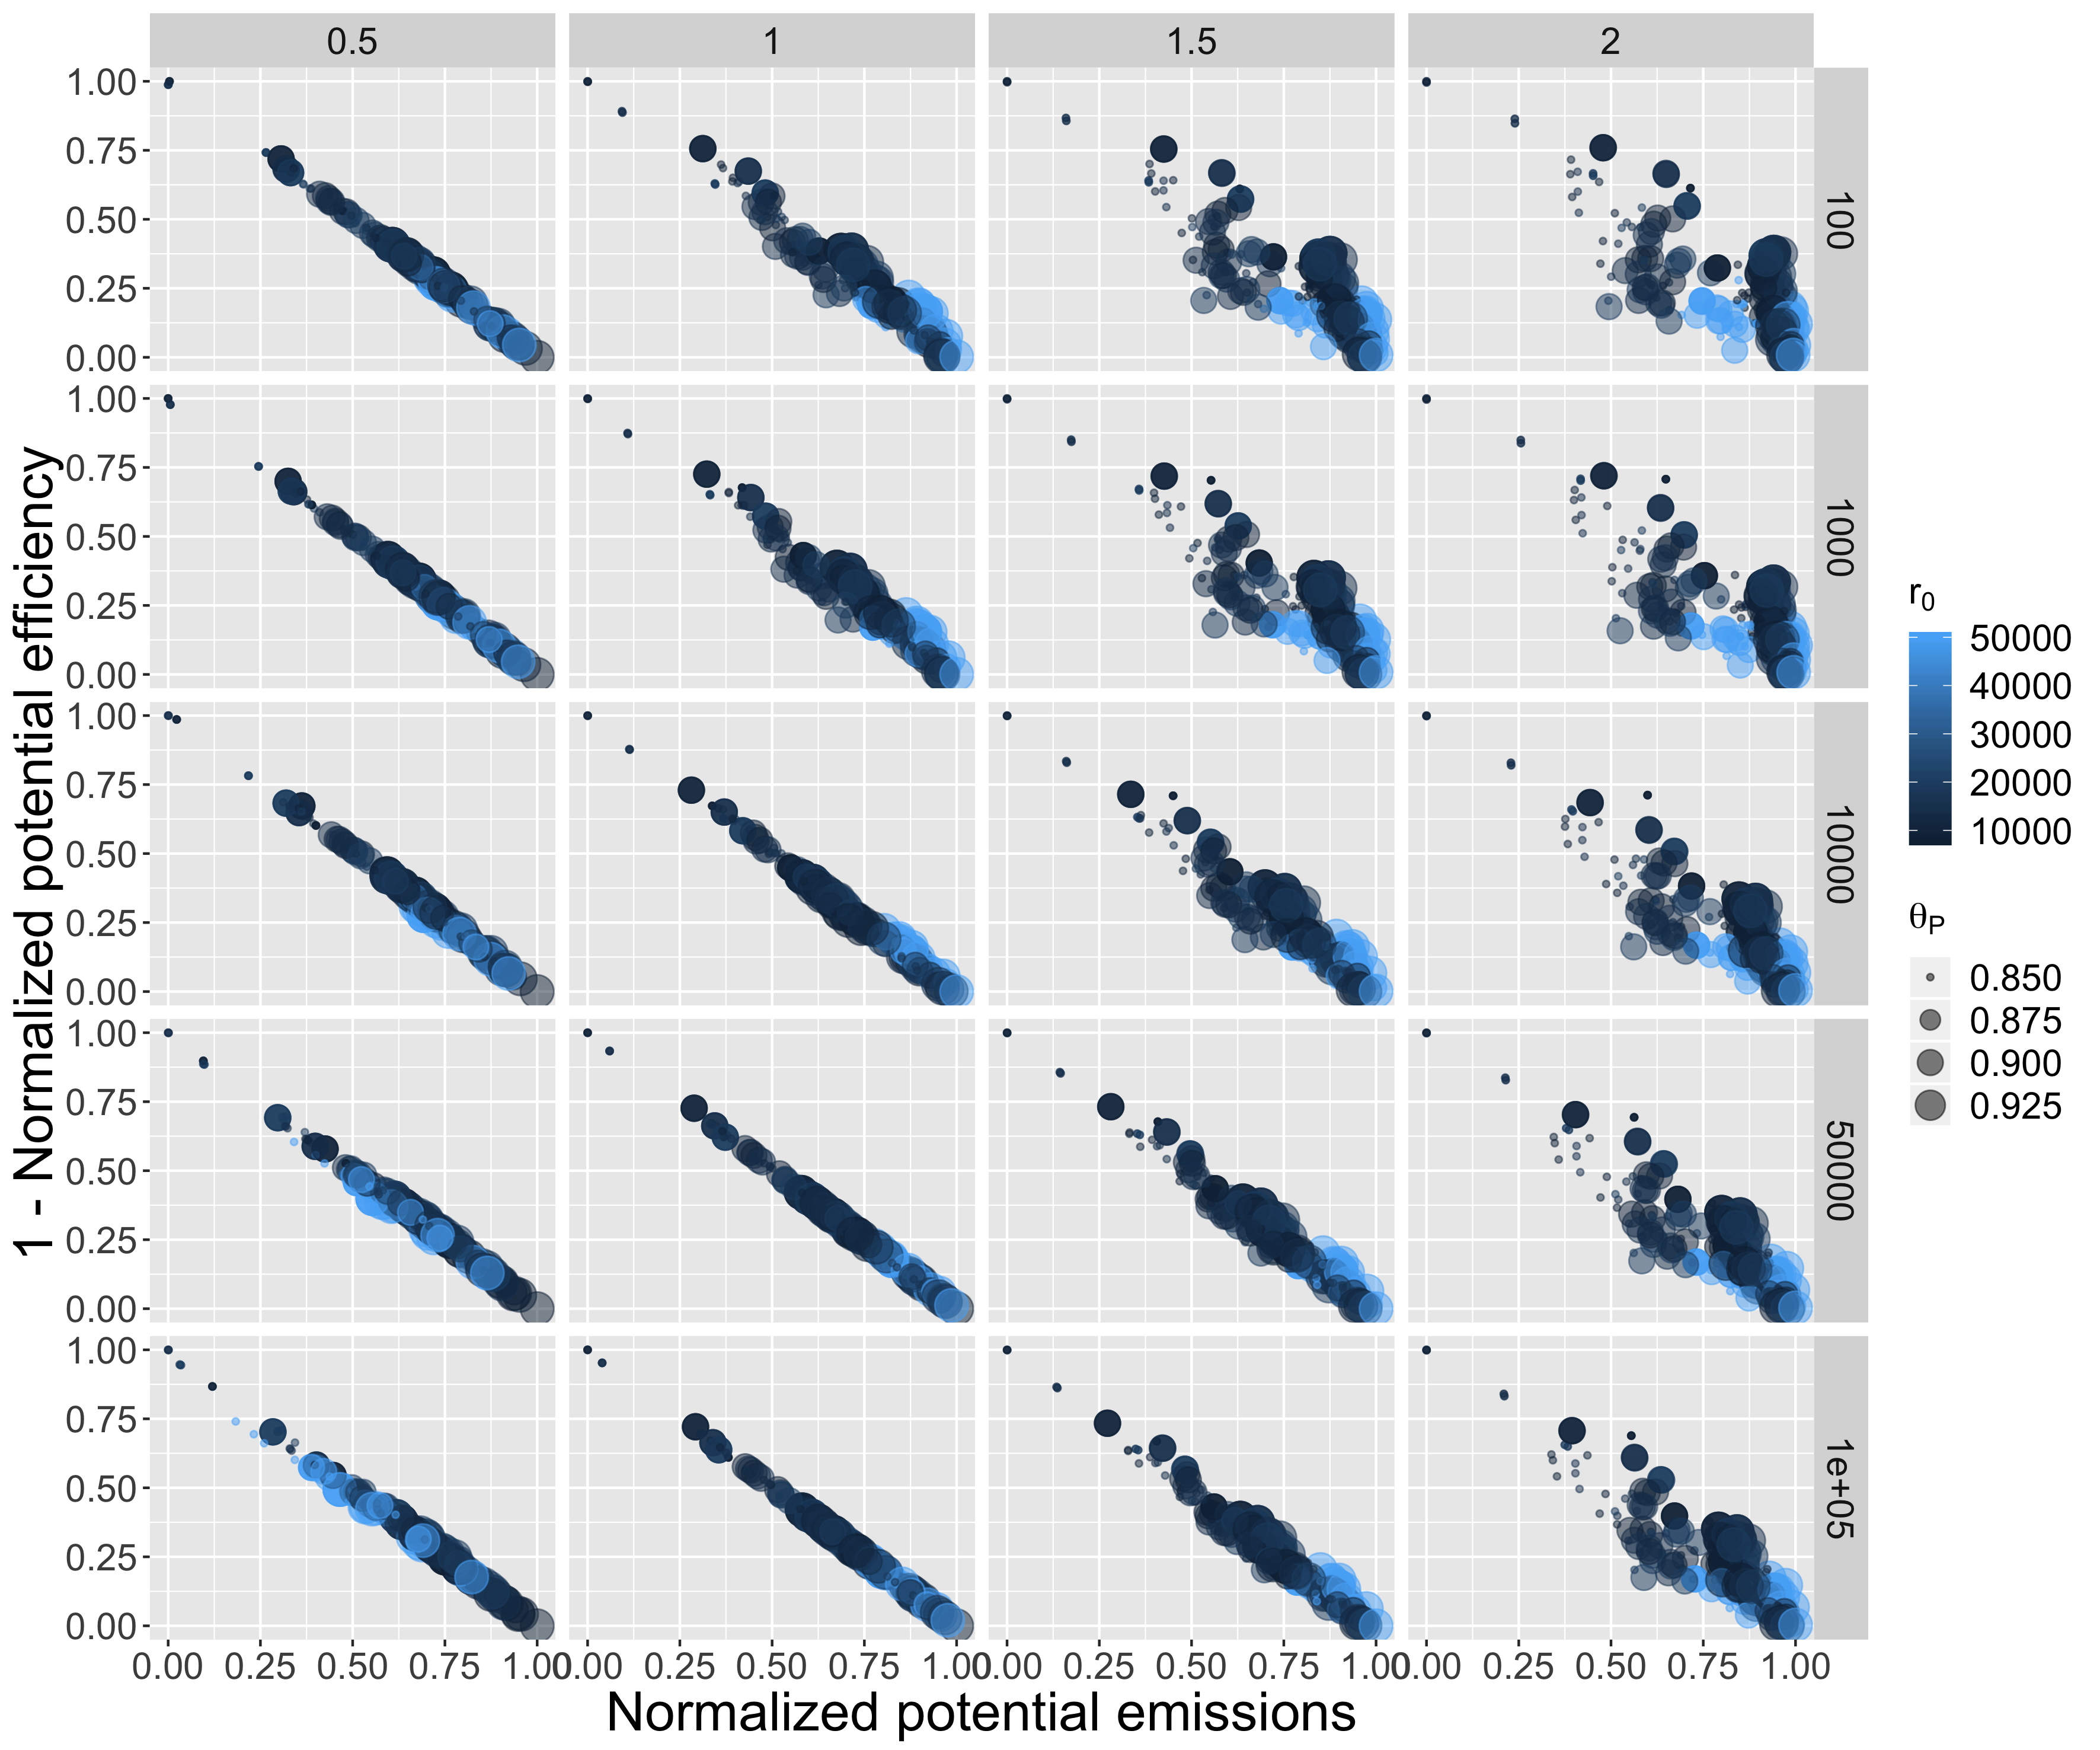
\includegraphics[height=0.8\textheight]{figures/aggreg_paretos_radiuspopthq.png}


}



\sframe{An optimal morphology ?}{

%# Cumulative Proportion  0.7296 0.9650 0.99761 1.00000
%                PC1       PC2         PC3         PC4
%moran   -0.3088585 0.9493848 -0.04444327  0.03605266
%avgdist  0.5417362 0.1415668 -0.82239570 -0.10072759
%entropy  0.5108424 0.2140447  0.45847647 -0.69499942
%slope    0.5917502 0.1811415  0.33390034  0.71100630

\textit{Optimal degree of monocentricity of the system for emissions.}

\centering

\medskip

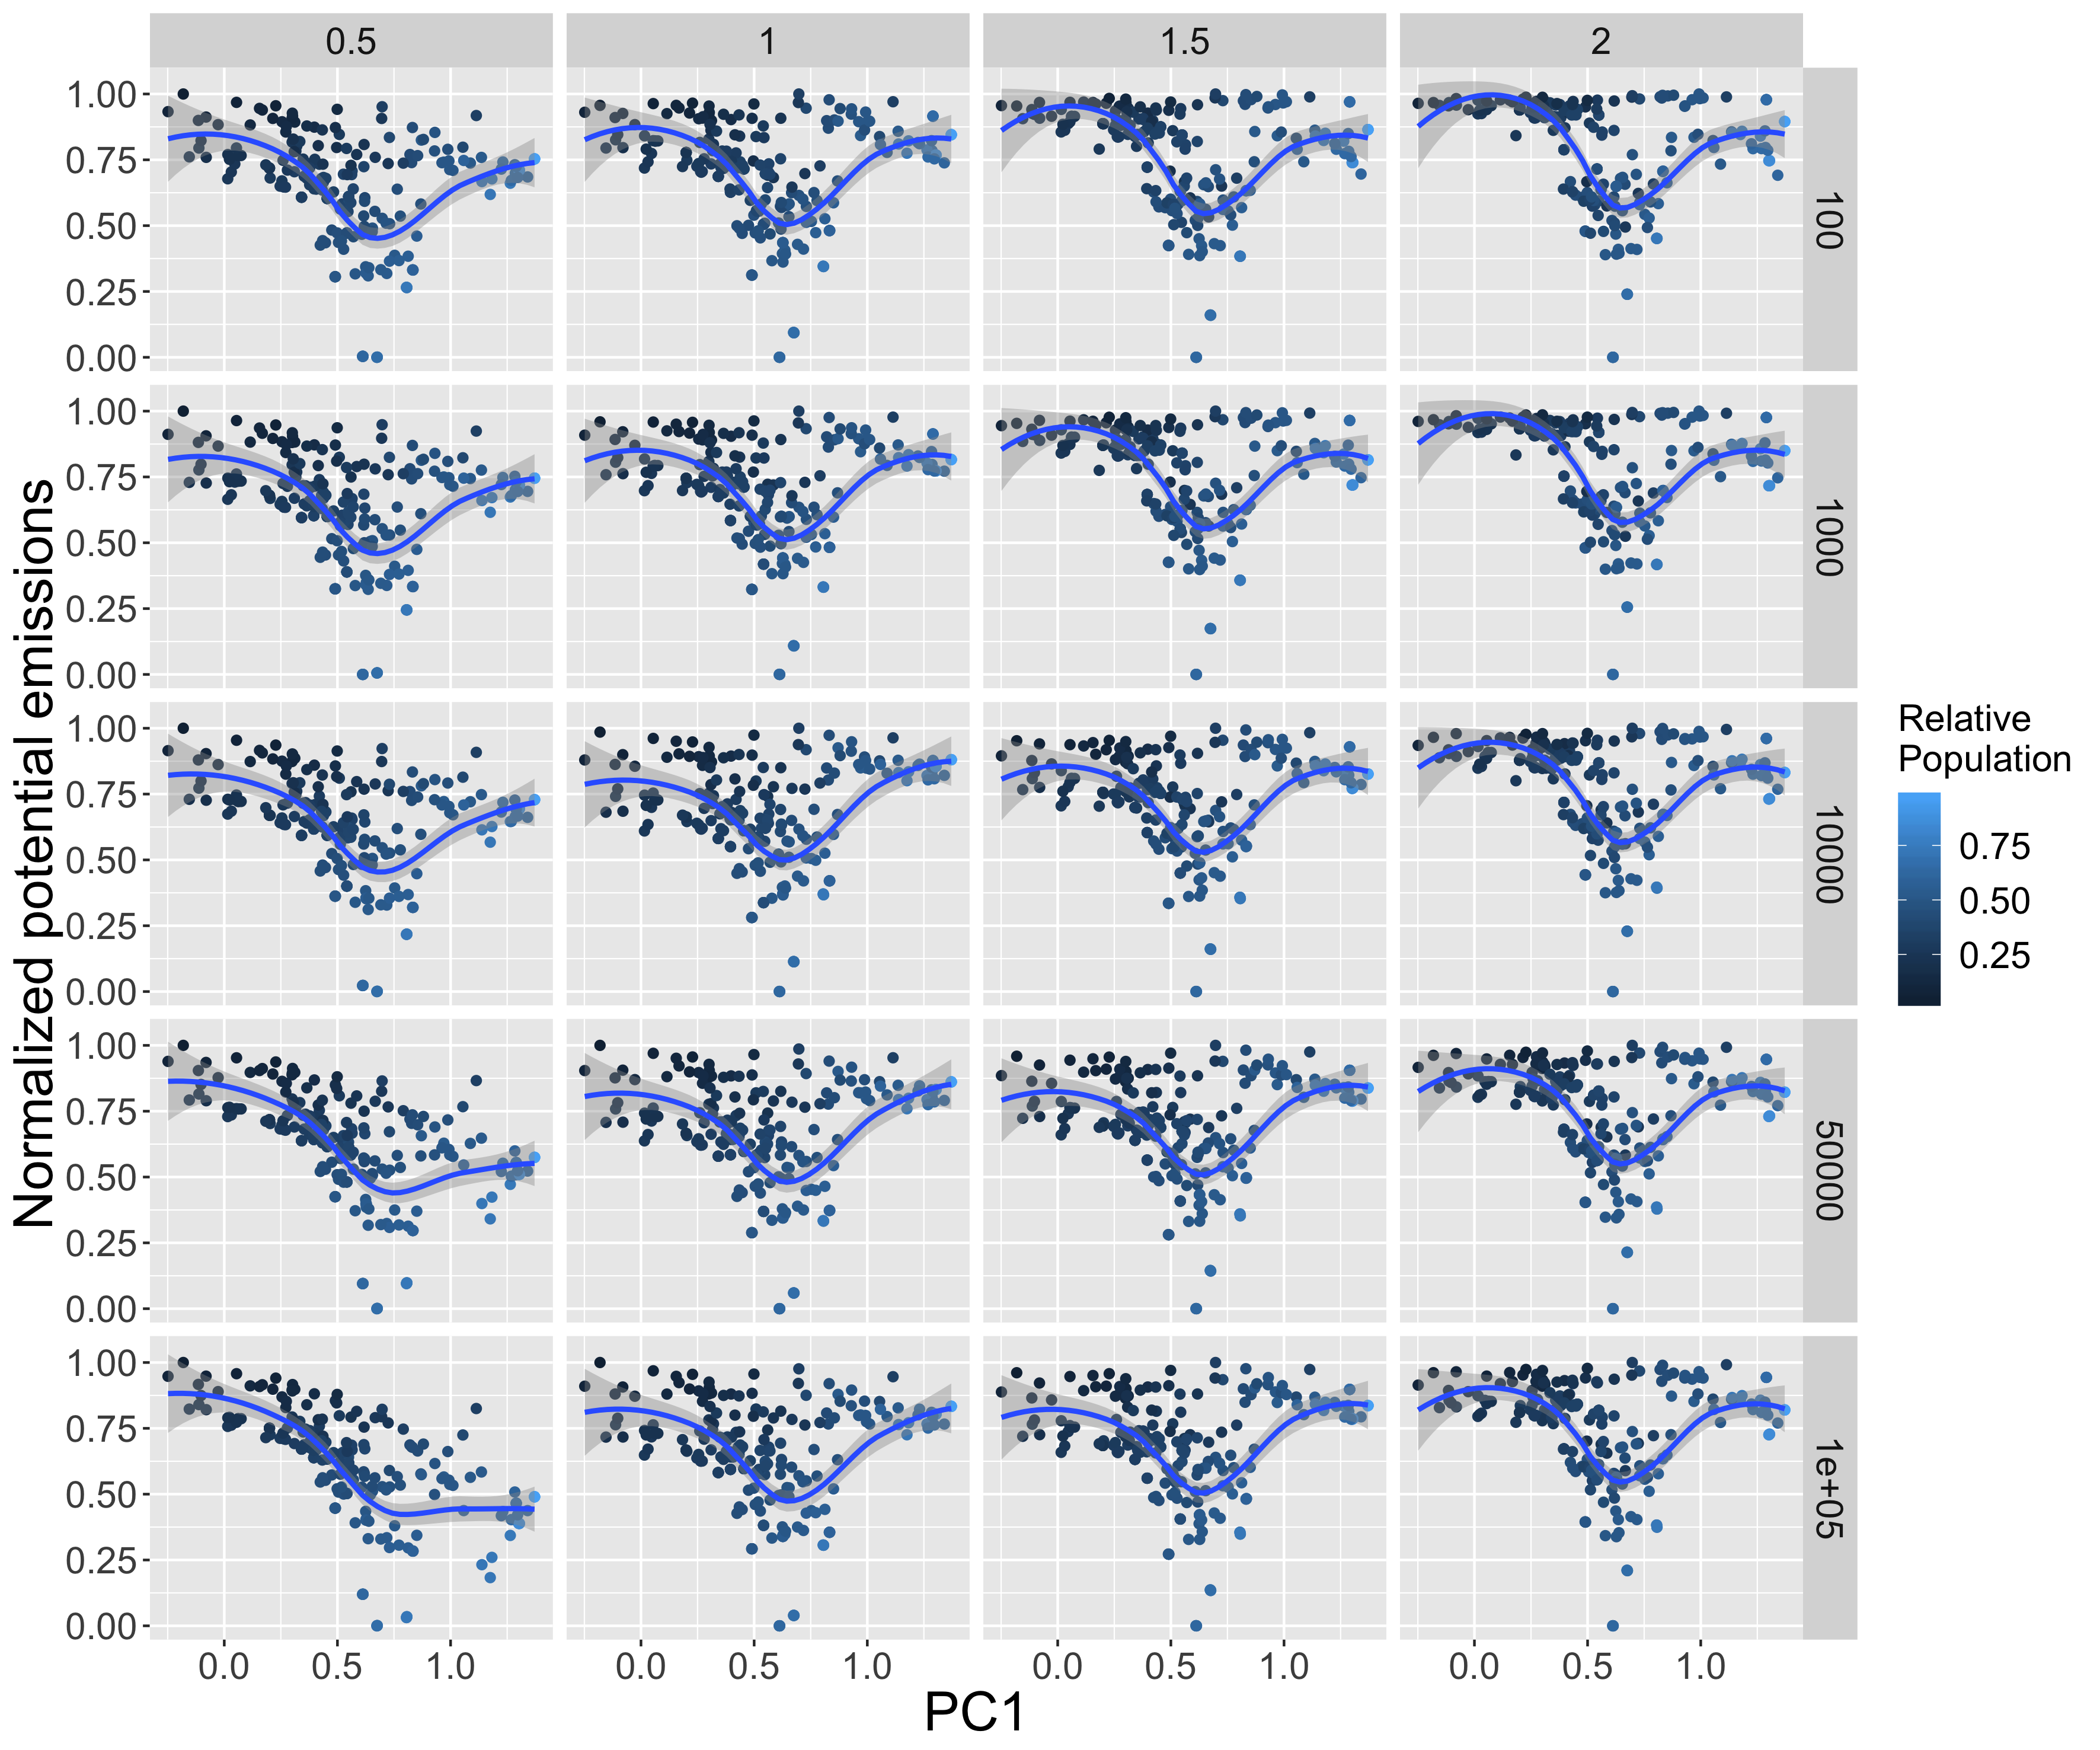
\includegraphics[height=0.85\textheight]{figures/aggreg_morpho_pc1-emissions.png}

}

\sframe{Morphological trade-offs}{

\vspace{-0.3cm}

\textit{No ``optimal'' cities, different forms yield different compromises in terms of relative indicators.}

\centering

\medskip

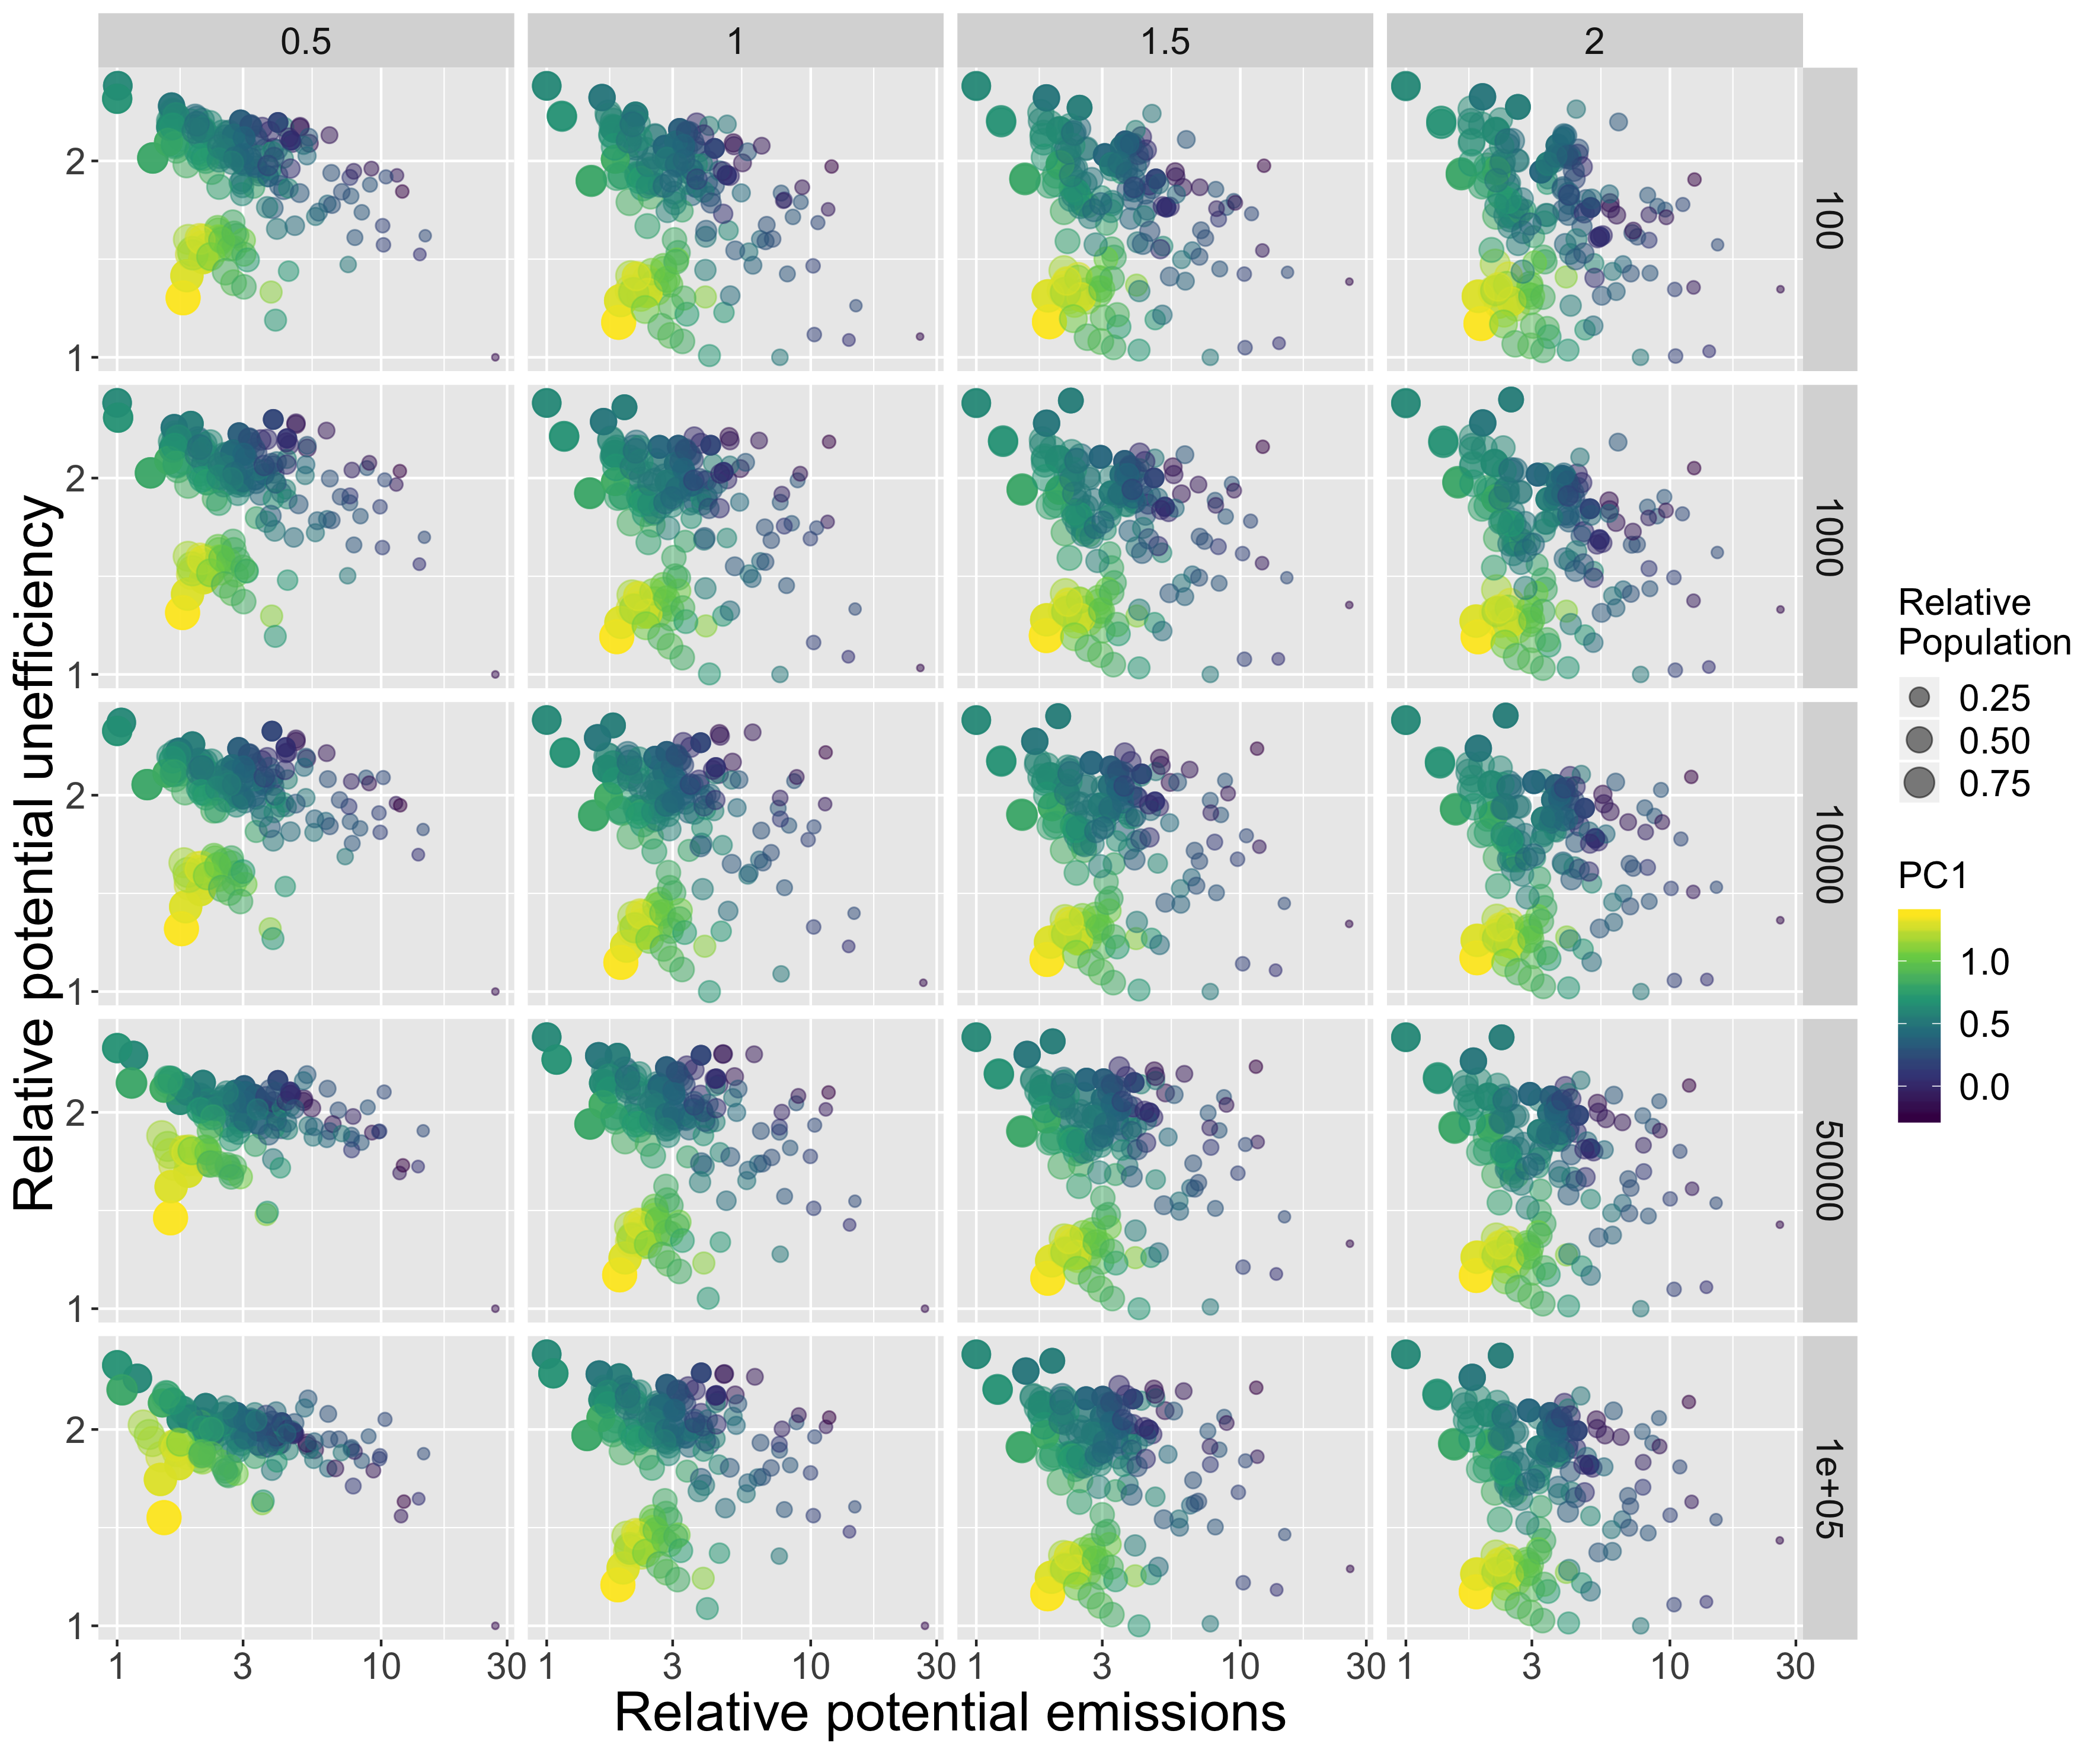
\includegraphics[height=0.83\textheight]{figures/aggreg_morpho_relemissions-relefficiency_colpc1_logscale.png}


}



\sframe{Towards a systematic calibration}{


% Further work will consist in the use of calibration heuristics \citep{reuillon2013openmole} to find in a more robust way optimal parameter values.

% -> depending on results


Grid sampling to explore regions rapidly limited

$\rightarrow$ towards the use of genetic algorithms on grid, made smooth with the OpenMOLE software \url{https://next.openmole.org/}

\centering

\smallskip


\includegraphics[height=0.35\textheight]{figures/openmole.png}

\smallskip

\raggedright\justify

\footnotesize \textit{OpenMOLE: (i) embed any model as a black box; (ii) transparent access to main High Performance Computing environments; (iii) model exploration and calibration methods.}

\bigskip

\textbf{Apply to the summer school !} \url{https://exmodelo.org/}

}




\sframe{Discussion}{

% This work paves the way towards ?


\justify

\vspace{-1cm}

\textbf{Implications}

\medskip

$\rightarrow$ Multi-dimensionality of urban systems and a link between form and function captured through multilayer percolation.
\smallskip

$\rightarrow$ Possible transfer to policy-making recommandations: Pareto-optimal configuration can be used for the planning of regional transportation networks, policies for subsidies, etc.

\bigskip



\textbf{Developments}

% 

% detail method to extrapolate parameters of gravity flows

% interesting result : compare these emission with the synthetic ? (then just a refinment ?) -> yes, better. show new Pareto fronts with this fixed parameters for only emissions, and varying for economic ? 

\medskip

$\rightarrow$ Systematic calibration of parameters to unveil more exhaustive Pareto fronts.

\smallskip

$\rightarrow$ Extrapolation of transportation flows to estimate potential emissions linked to transportation: calibration of gravity model on actual transportation emissions; use of the extrapolated parameters in potentials.

\smallskip

$\rightarrow$ More refined indicators for sustainability (socio-economic integration, accessibilities, different scaling exponents).
% ex : at least different scaling exponent.


}



\sframe{Conclusion}{


\justify

\vspace{-0.8cm}

% rq : try in all conclusion to come back to these points, close to Banos commadments ?

$\rightarrow$ Empirical and theoretical research directed towards concrete policy-making applications. \textbf{Need for more data-driven approaches.}
%First step towards systematic benchmarks and multi-modeling. \textbf{Need for more systematic model exploration.} % model coupling / benchmarking

\smallskip

$\rightarrow$ Towards multi-scalar approaches ? \textbf{Need for more integrated models.}
 %Model integration and multi-scalarity ? \textbf{Need for more integrated models.}

\smallskip

$\rightarrow$ Multidimensionality of urban systems ? \textbf{Need for more interdisciplinarity.}

\bigskip

\footnotesize

\textbf{Related works}


Raimbault, J. (2018). Calibration of a density-based model of urban morphogenesis. PloS one, 13(9), e0203516.

\smallskip	

Raimbault, J. (2018). An Urban Morphogenesis Model Capturing Interactions between Networks and Territories. \textit{Forthcoming in Mathematics or Urban Morphogenesis.} arXiv:1805.05195.

\smallskip


Raimbault, J. (2018). Caract{\'e}risation et mod{\'e}lisation de la co-{\'e}volution des r{\'e}seaux de transport et des territoires (Doctoral dissertation, Université Paris 7 Denis Diderot). \url{https://halshs.archives-ouvertes.fr/tel-01857741}




\medskip

\textbf{Open repository} at \texttt{https://github.com/JusteRaimbault/UrbanMorphology} (code, data and results)%\\\smallskip

% no grid used
%\textbf{Acknowledgments}: thanks to the \textit{EGI} for access to the infrastructure.


}






\sframe{Reserve slides}{

\centering

\Large

\textbf{Reserve Slides}

}


\sframe{Results: effective emissions}{

\textit{Effective emissions exhibit a supralinear scaling of population}

\medskip

\centering

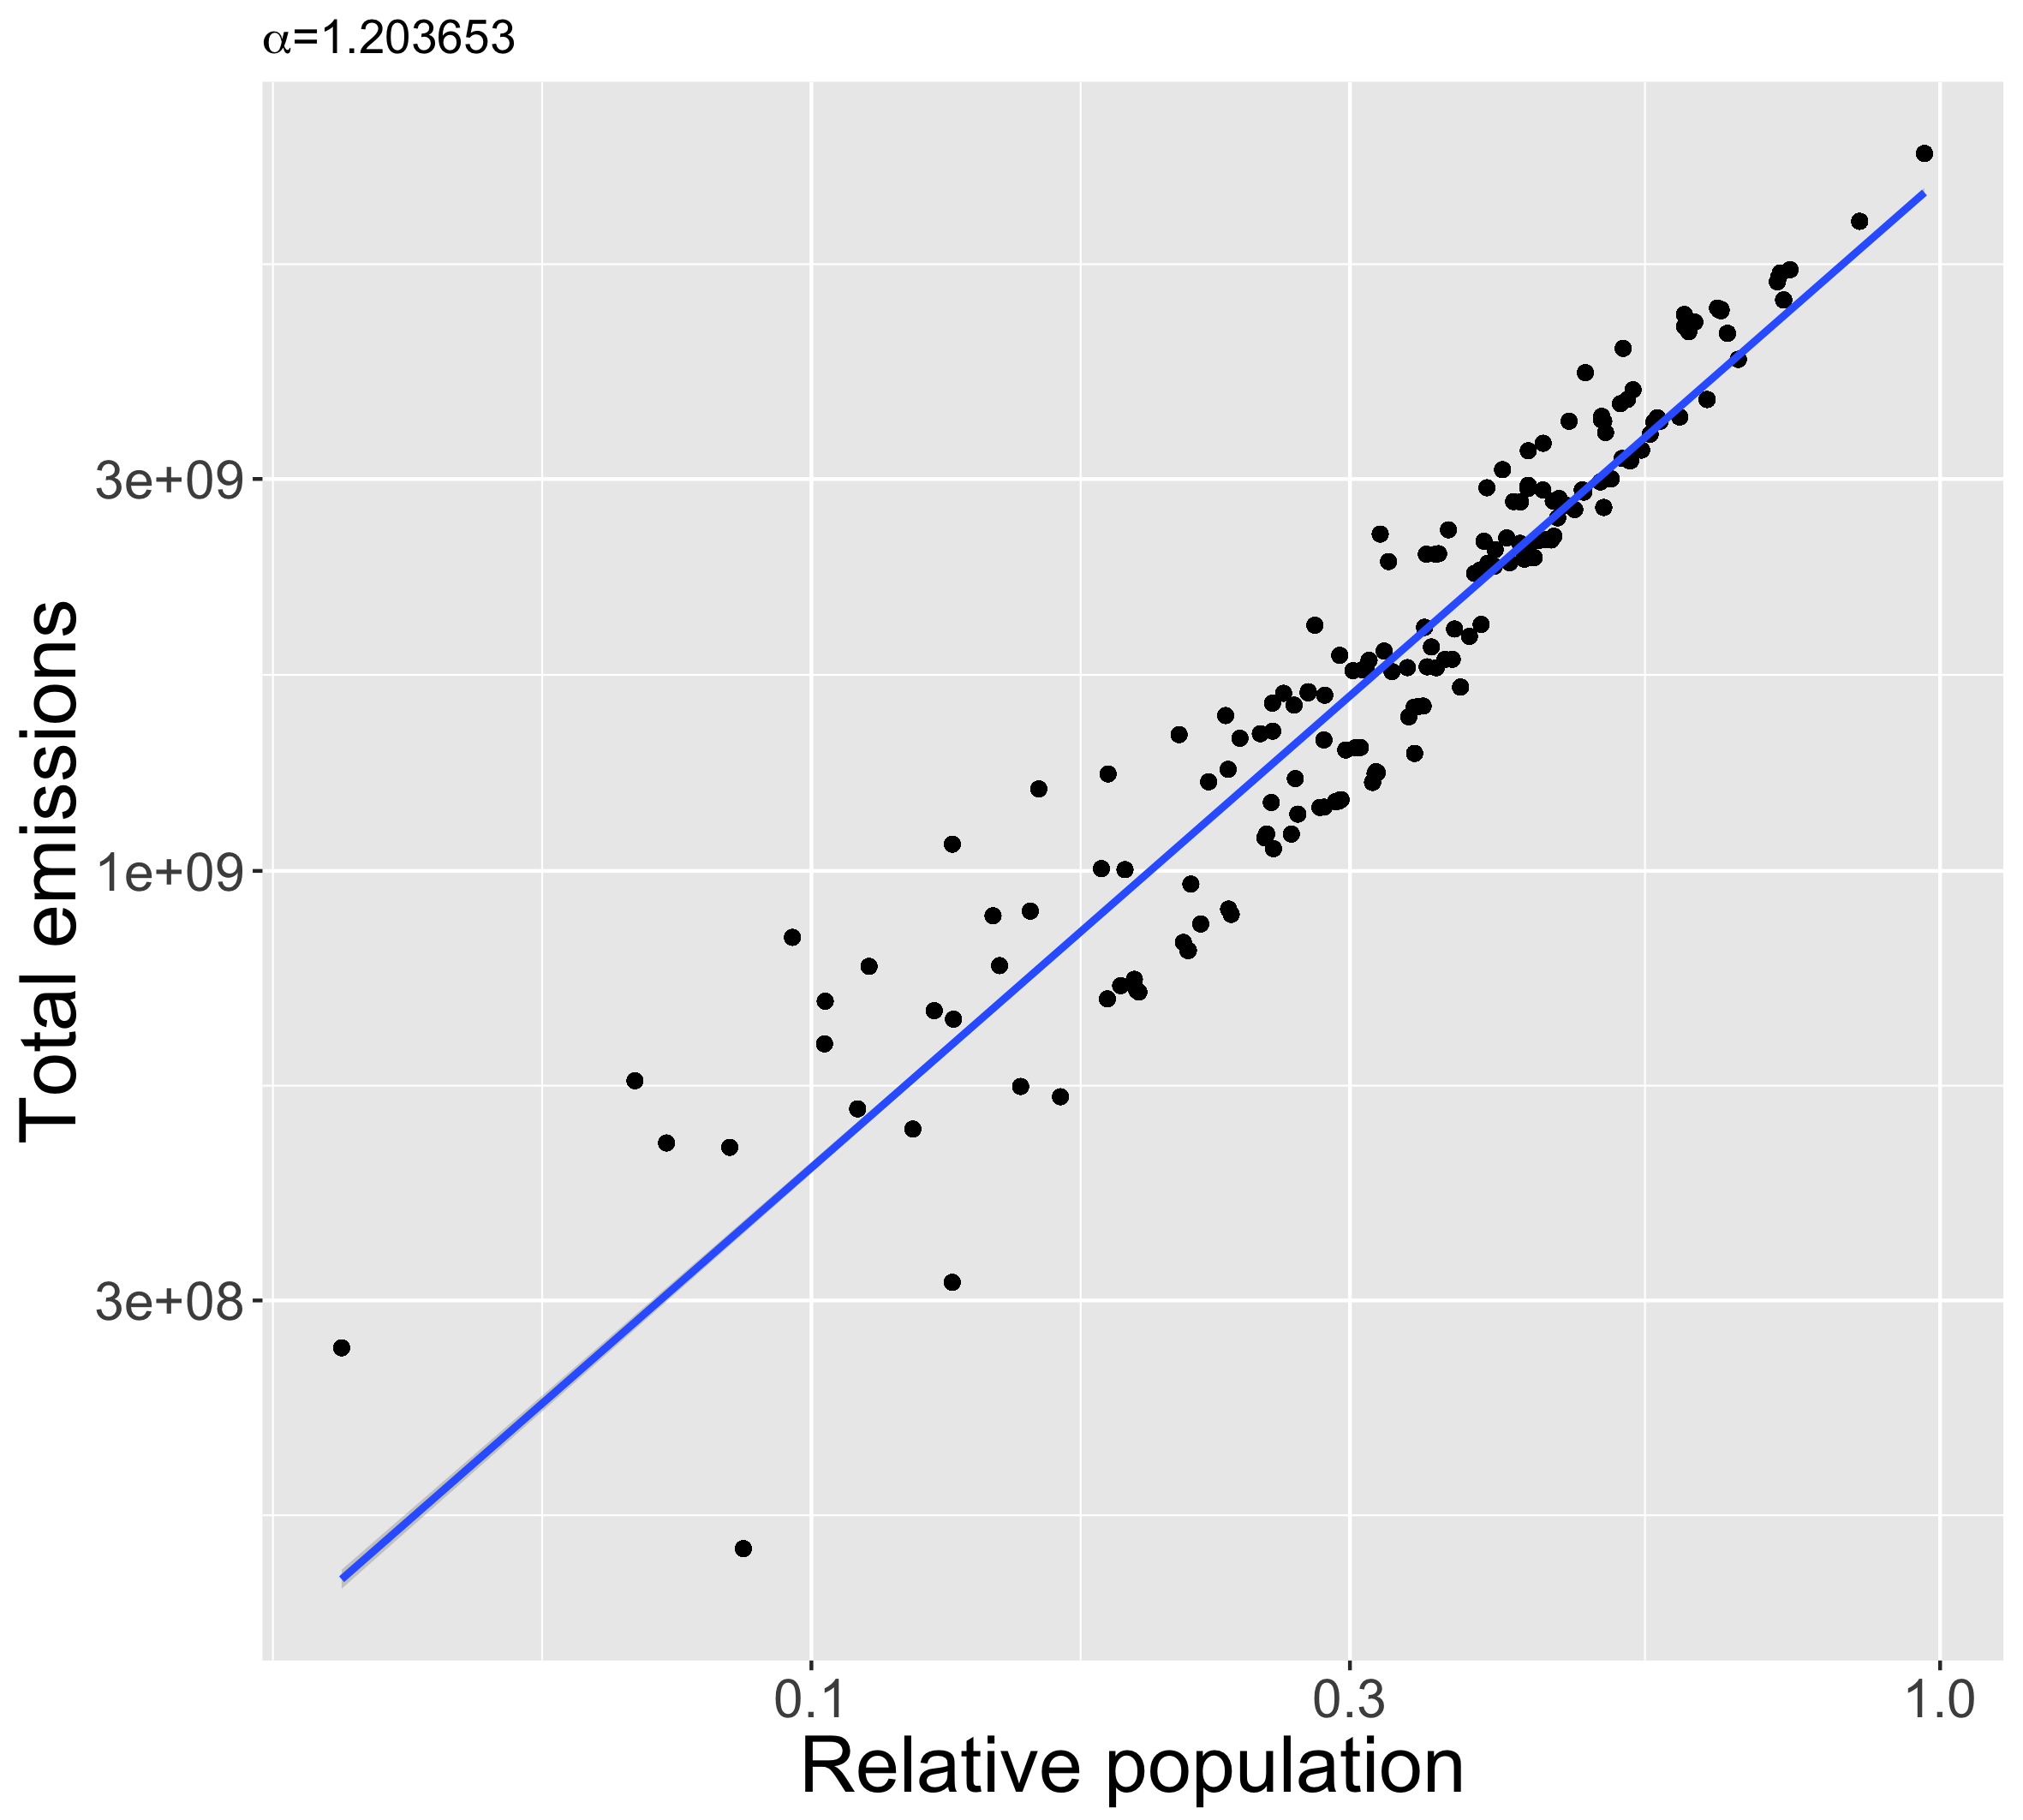
\includegraphics[height=0.83\textheight]{figures/aggreg_effective.png}

}

\sframe{Results: all clusters Pareto fronts}{

\textit{Variation of Pareto front patterns when potential parameter $\gamma,d_0$ vary.}

\medskip

\centering

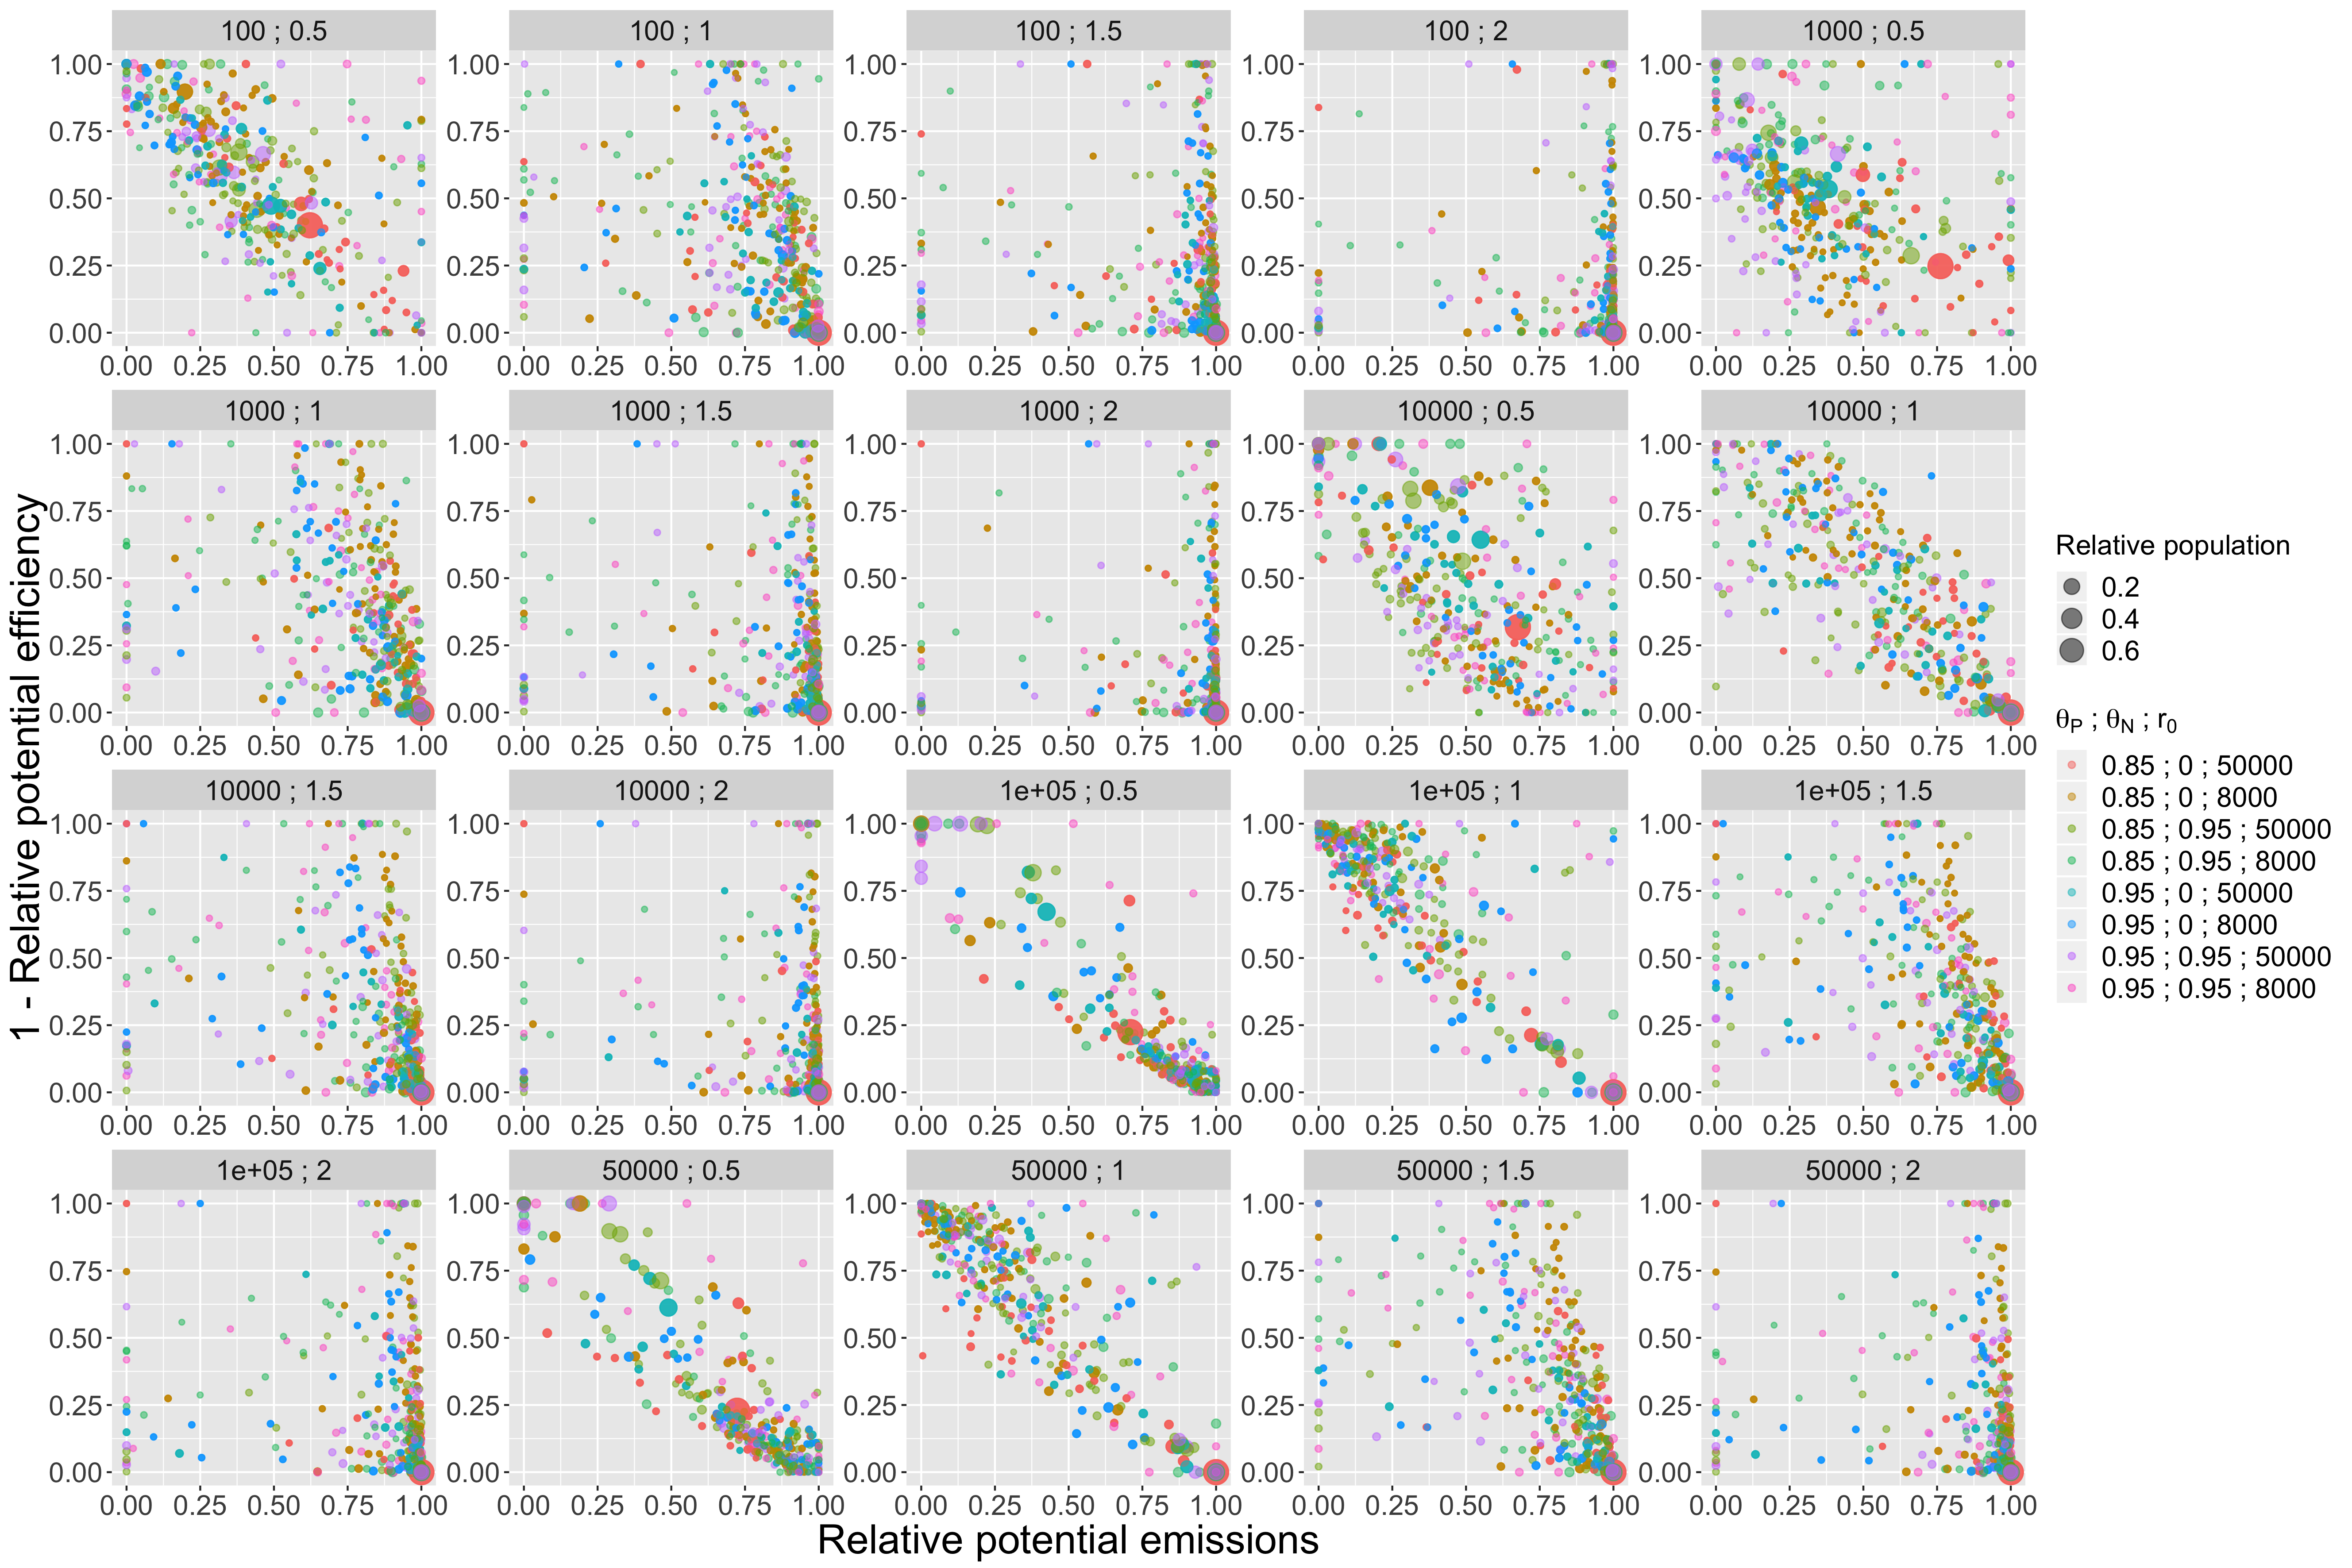
\includegraphics[width=0.9\textwidth]{figures/full_paretos.png}

}


\sframe{Results: an optimal morphology}{

\textit{More monocentric areas are more optimal in terms of relative emissions and efficiency ?}

\medskip

\centering

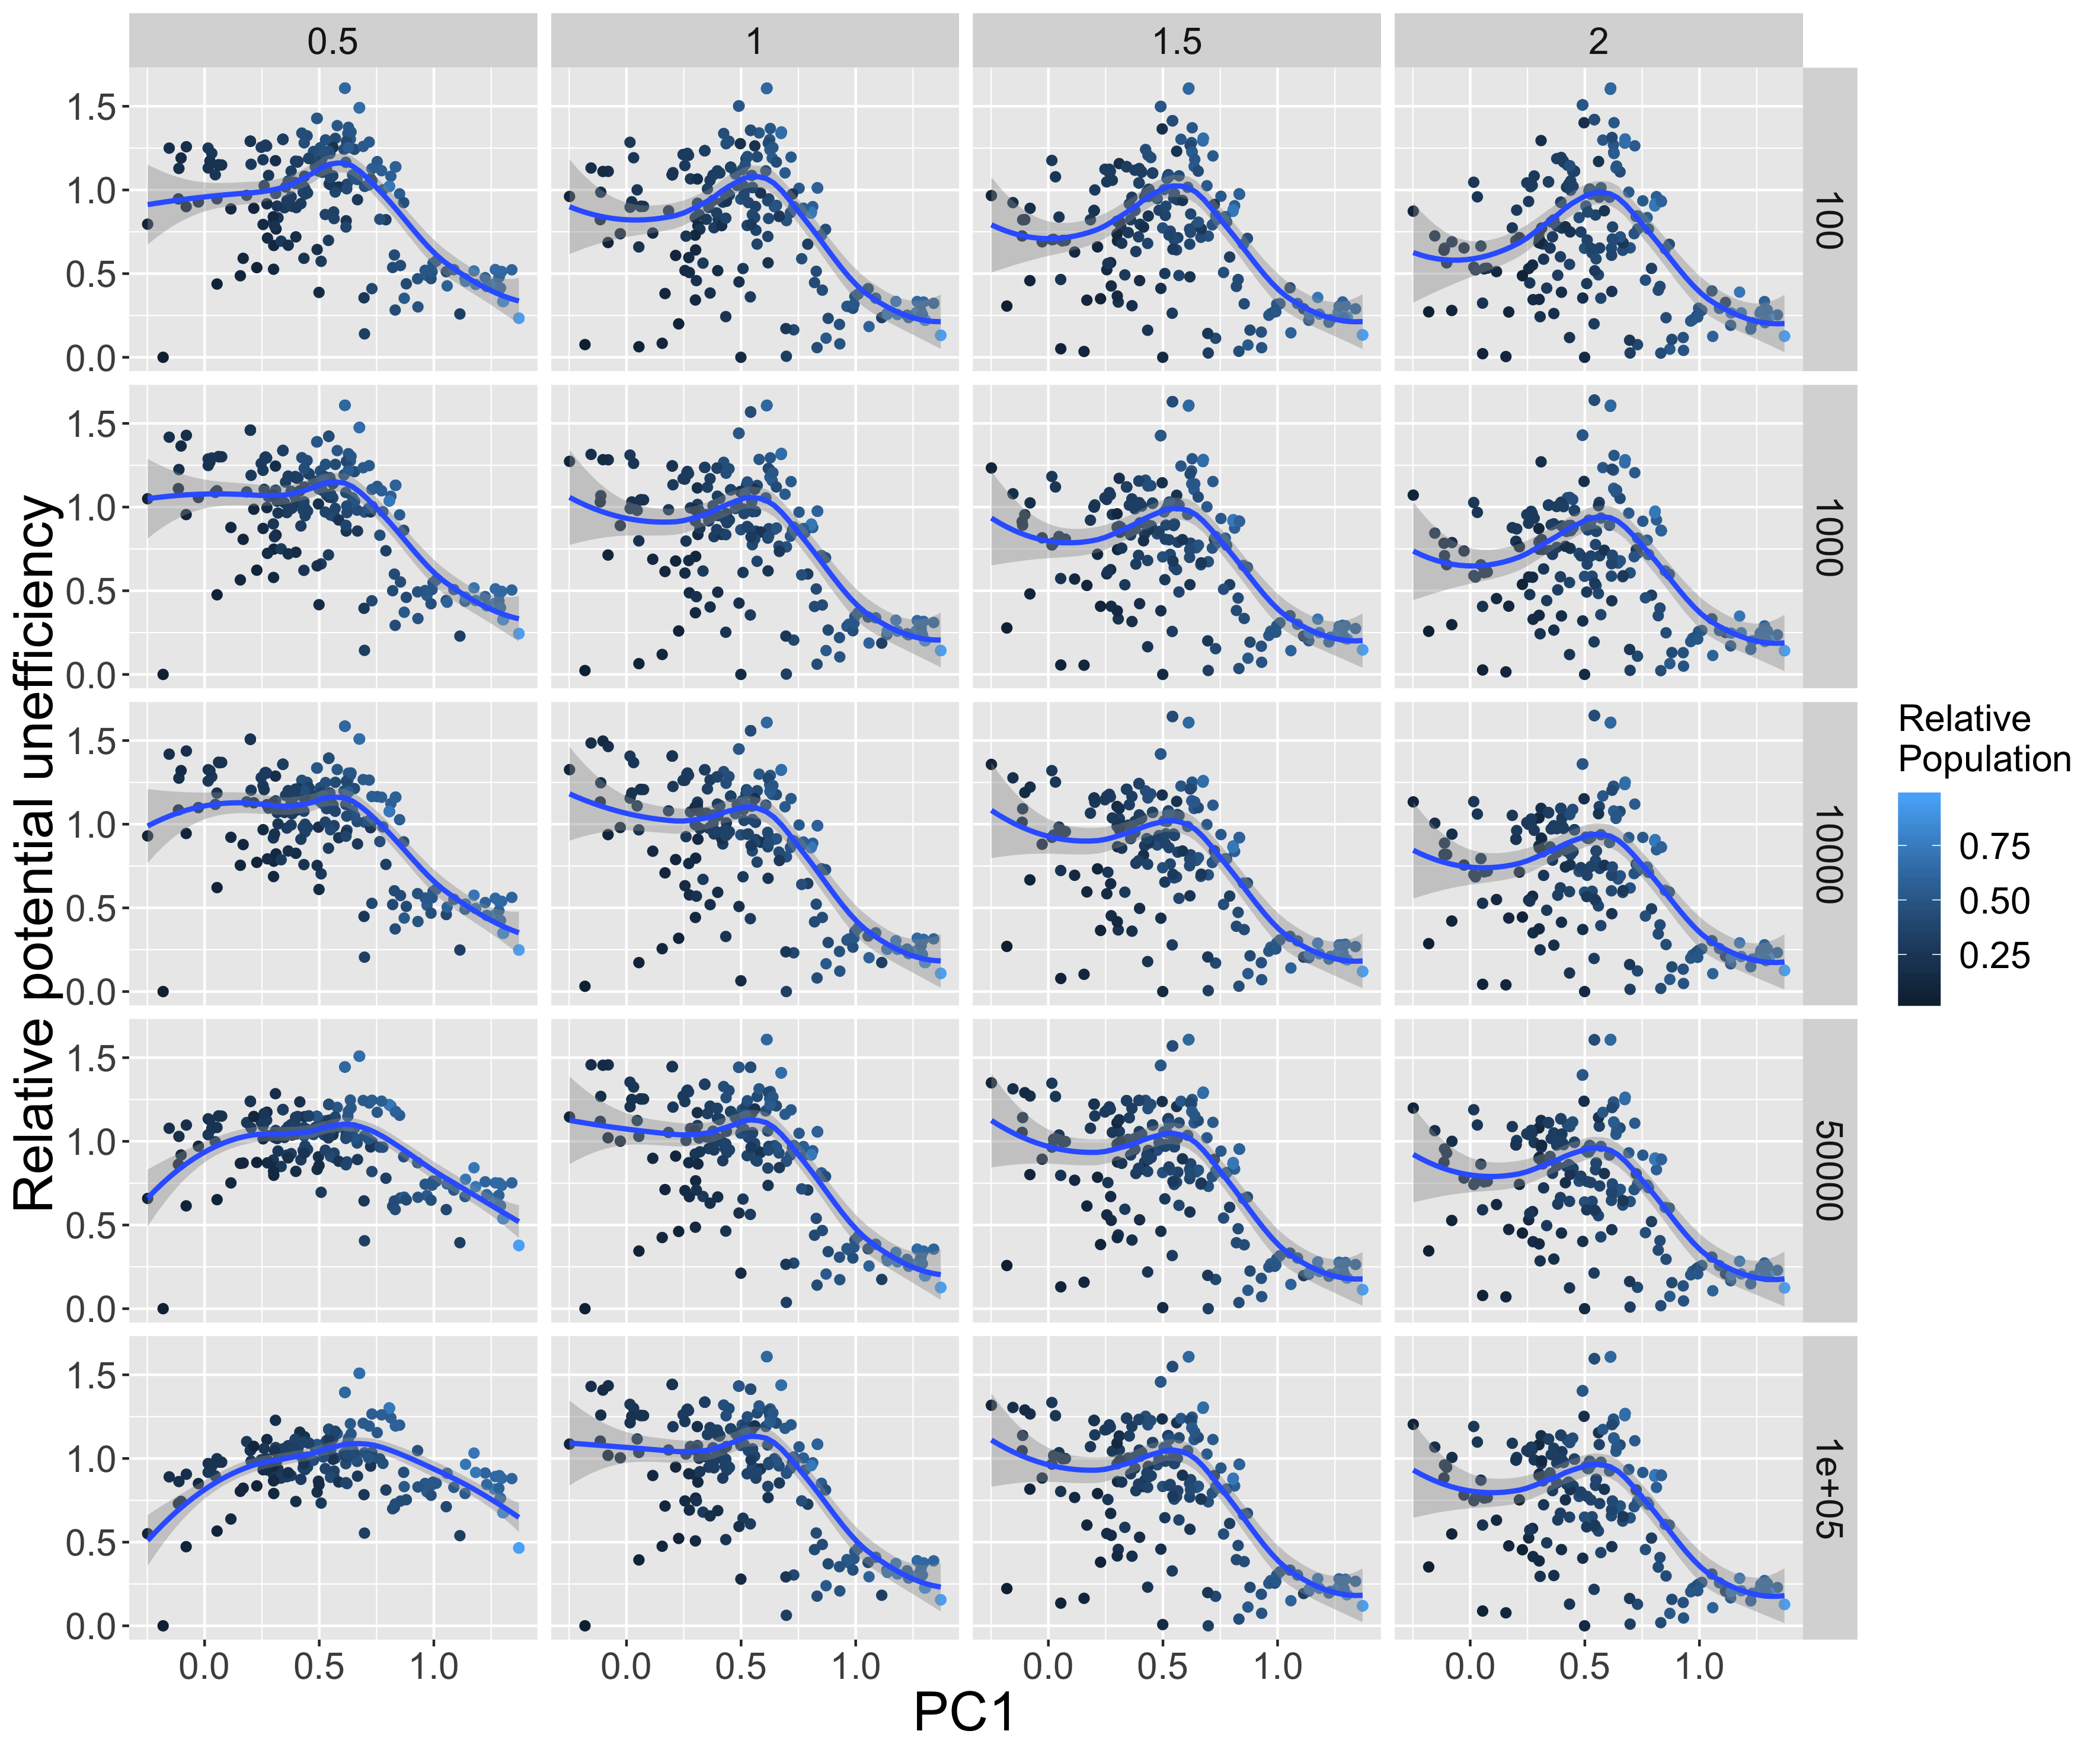
\includegraphics[width=0.49\textwidth]{figures/aggreg_morpho_pc1-relefficiency.png}
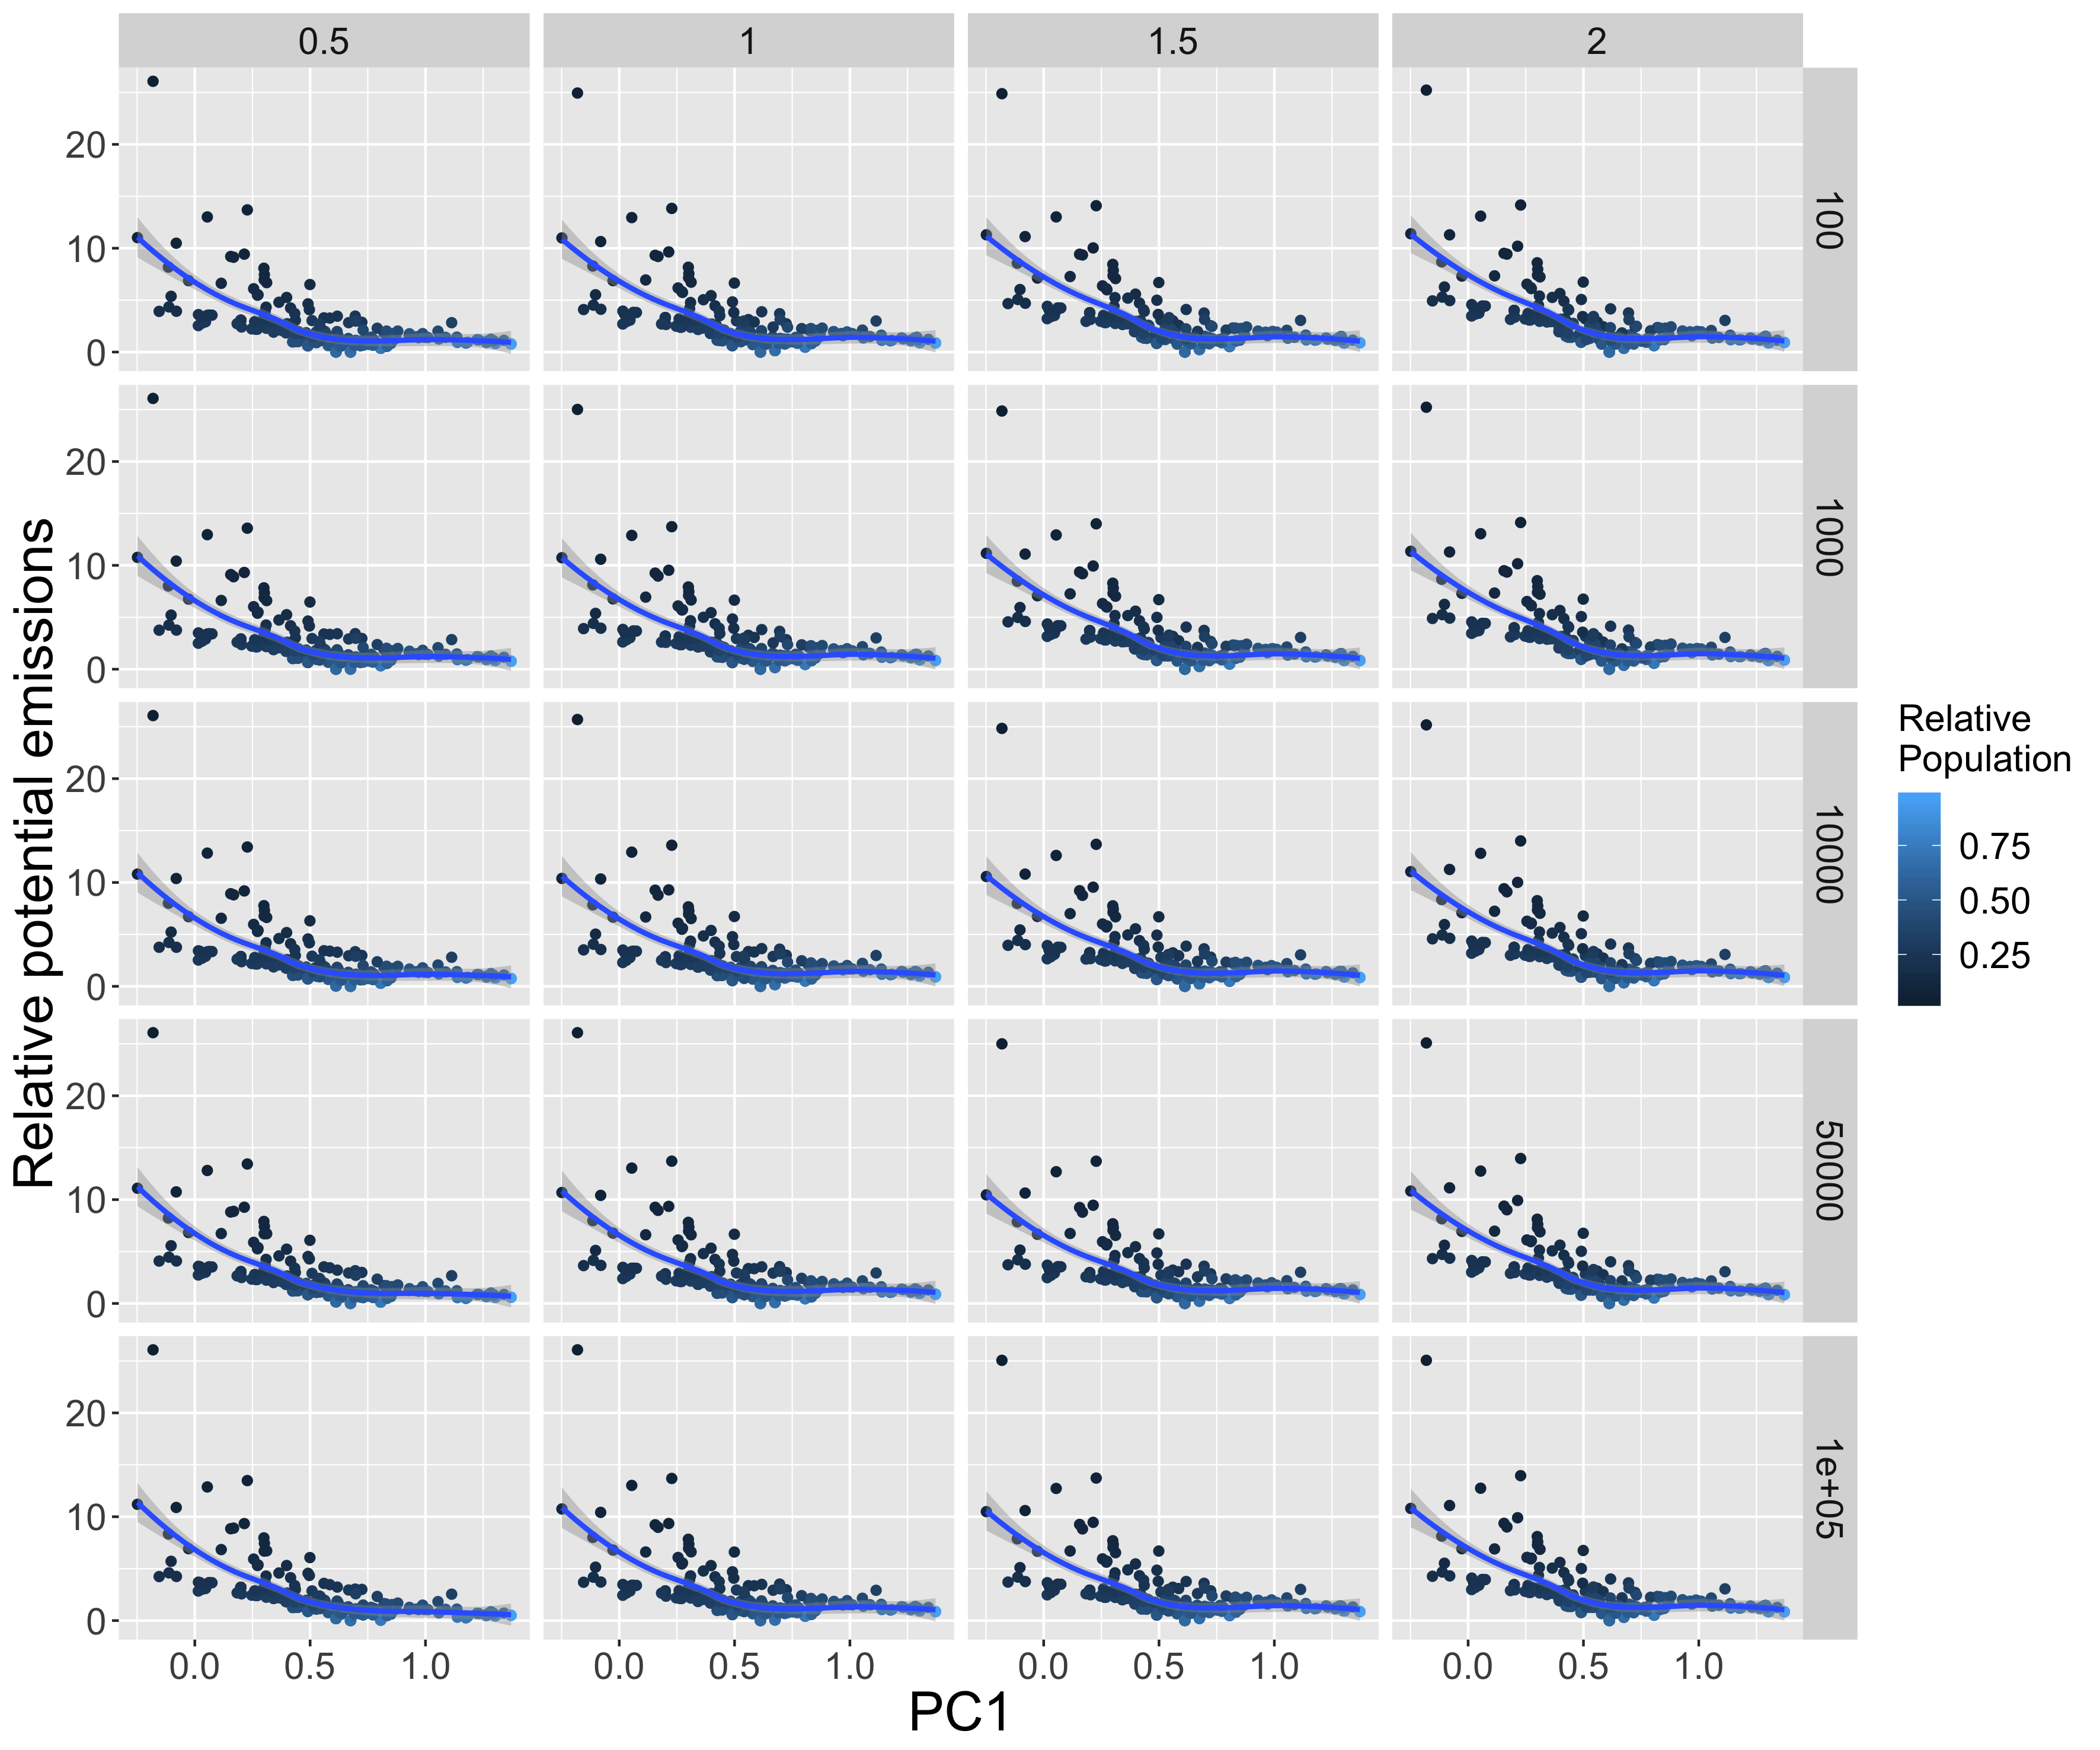
\includegraphics[width=0.49\textwidth]{figures/aggreg_morpho_pc1-relemissions.png}

% TODO : curves for emissions rescale to the same -> link with Caruso profiles ? ; investigate that, and why not for efficiency.


}




%%%%%%%%%%%%%%%%%%%%%
\begin{frame}[allowframebreaks]
\frametitle{References}
\bibliographystyle{apalike}
\bibliography{/Users/juste/ComplexSystems/CityNetwork/Biblio/Bibtex/CityNetwork,biblio}
\end{frame}
%%%%%%%%%%%%%%%%%%%%%%%%%%%%




\end{document}









